% !TeX root = ../main.tex
\chapter{Numerical results: preliminary investigation}
\label{chapt:results_preliminary}

\section{Inversion of the Dirac operator}
\begin{figure}[h]
    \centering
    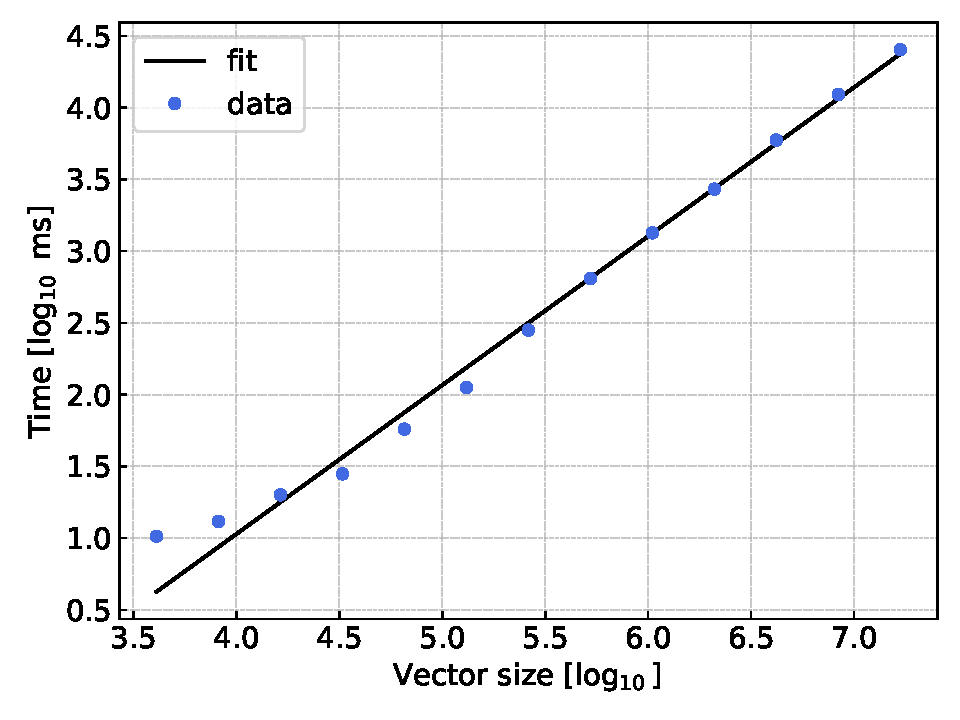
\includegraphics[scale=0.65]{figures/complexity.pdf}
    \caption{}
    \label{fig:complexity}
\end{figure}

\section{The fermionic correlator}
To start with the study of the model, we want to analyse the behaviour of the fermionic correlator and illustrate the fermionic masses extraction procedure. \\
Let us initially restrict to $g = 0$, so that the Dirac operator reduces to the one of free Wilson fermions \textcolor{red}{ref eq.}
\raggedright We then compute the correlator numerically via a single inversion of the Dirac operator as detailed in Appendix \ref{chap:AppendixC}. The lattice volume is chosen to be $128 \times 128$. \\
Figure \ref{fig:correlator_mass} reports the fermionic correlator as a function of $m_q$. One can see that a bigger bare quark mass results in a quicker decay, in accordance with the decay law \textcolor{red}{ref. eq.}. On the other side, a smaller mass results in a slower decay and tends to deform the characteristic shape of the correlator. \\~\\
\begin{figure}[h]
    \centering 
    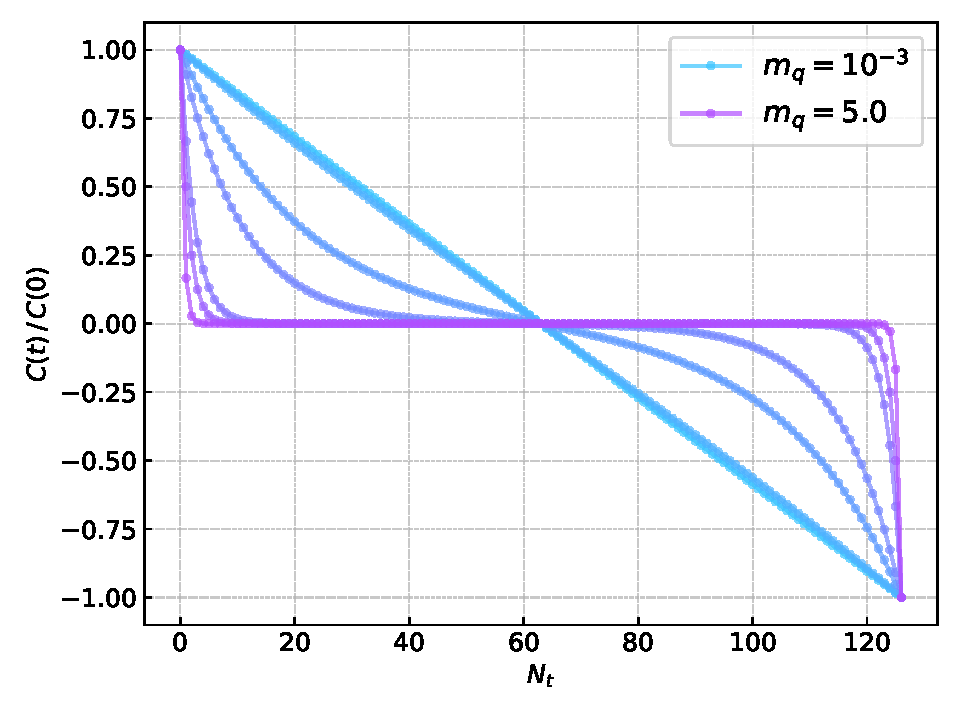
\includegraphics[scale=0.6]{figures/correlator/correlator.pdf}
    \caption[Fermionic correlator]{Normalised fermionic correlator for different values of the bare quark mass. A bigger mass results in a quicker decay, according to \textcolor{red}{eq. ref.}}
    \label{fig:correlator_mass}
\end{figure}
Figure \ref{fig:correlator_CGiter} shows the number of iterations needed for convergence of the Conjugate Gradient algorithm. While the exact number depends on the desired tolerance, one can clearly see that the number of iterations grows as $m_q \to 0$, due to an increase in the condition number \cite{cond_num_ref}. \\
\begin{figure}[h]
    \centering 
    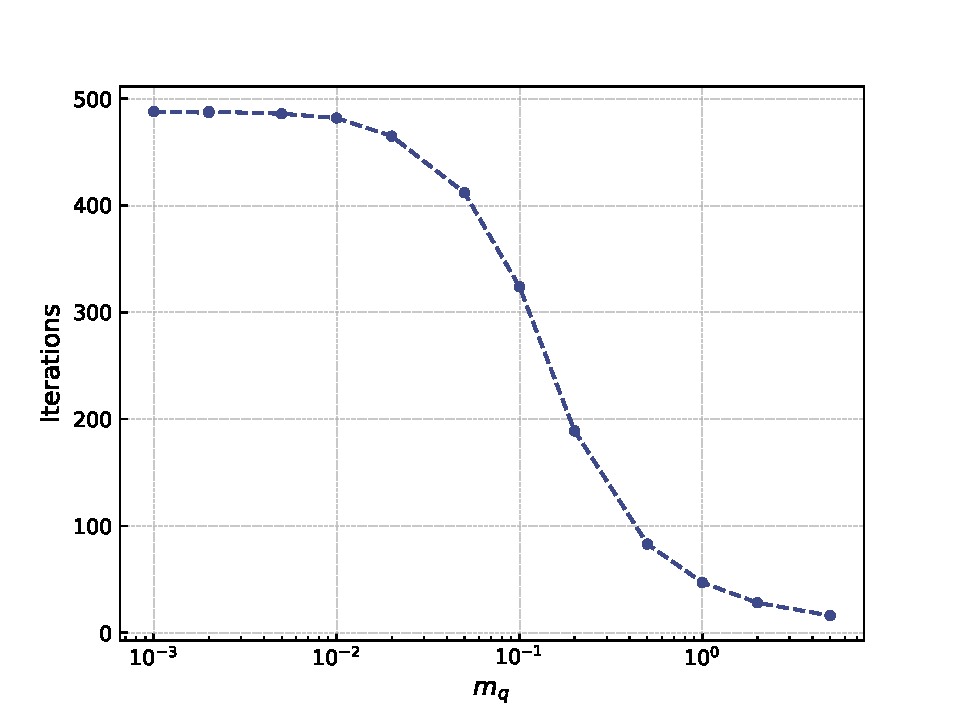
\includegraphics[scale=0.6]{figures/correlator/CGiter.pdf}
    \caption{CG iterations}
    \label{fig:correlator_CGiter}
\end{figure} 
\newpage
For the Dirac operator \textcolor{red}{ref eq.}, one can derive an analytical expression for the fermionic mass. The Dirac operator in momentum space reads \textcolor{red}{non lo hai mai introdotto}
\begin{equation*}
\bar{D}(p)= m_q + \sum_\mu 2 \sin ^2\left(\frac{p_\mu}{2}\right)+i \sum_\mu \gamma_\mu \sin \left(p_\mu\right)
\end{equation*}
and its inverse is
\begin{equation*}
    \bar{D}^{-1}(p) = \frac{m_q + \sum_\mu 2 \sin ^2\left(\frac{p_\mu}{2}\right) - i \sum_\mu \gamma_\mu \sin \left(p_\mu\right)}{m_q + \sum_\mu 2 \sin^2\left(\frac{p_\mu}{2}\right) + \sum_\mu \sin^2 \left(p_\mu\right)}.
\end{equation*}
One can now find the pole by imposing the numerator evaluated at $p^\mu =(im_\text{phys}, 0)$ to zero:
\begin{equation*}
    \left[m_q + \sum_\mu 2 \sin ^2\left(\frac{p_\mu}{2}\right)\right]^2_{p_\mu = (im_\text{phys}, 0)} + \left[\sum_\mu \gamma_\mu \sin \left(p_\mu\right)\right]^2_{p_\mu = (im_\text{phys}, 0)} = 0.
\end{equation*}
This results in a trascendental equation 
\begin{equation*}
    \left[m_q - 2 \sinh^2\left(\frac{m_\text{phys}}{2}\right)\right]^2 - \sinh^2\left(m_\text{phys}\right) = 0,
\end{equation*}
which has the solution 
\begin{equation}
    m_\text{phys} = \log\left(1+m_q\right).
    \label{eq:analytical_wilson}
\end{equation}
We then choose three values of the bare quark mass, compute the correlator numerically and perform a fit according to \eqref{eq:correlator_mass_extraction}, in order to extract the physical mass. We then compare it to the theoretical value given by \eqref{eq:analytical_wilson}. The results are reported in figures \ref{fig:fit_wilson} and table \ref{tab:free_wilson_fit}. \\~\\
\begin{table}
    \centering
    \begin{tabular}[pos]{ccc}
        \toprule
        $m_q$ & teo & fit \\
        \midrule 
        1.0 & 0.6931471805599453 & 0.6931537171644739 \\
        0.1 & 0.09531017980432493 & 0.09531020915059212 \\
        0.01 & 0.009950330853168092 & 0.009950277657505842 \\
        \bottomrule
    \end{tabular}
    \caption[Fit of the correlator for free Wilson fermions.]{The correlator for free Wilson fermions is fitted to \textcolor{red}{(eqref)} and compared to its analytical value given by \eqref{eq:analytical_wilson}. The precision for the Conjugate Gradient algorithm was set to $r^2 \leq 10^{-10}$.}
    \label{tab:free_wilson_fit}
\end{table}
\begin{figure}
    \centering
    \begin{subfigure}[b]{0.48\textwidth}
        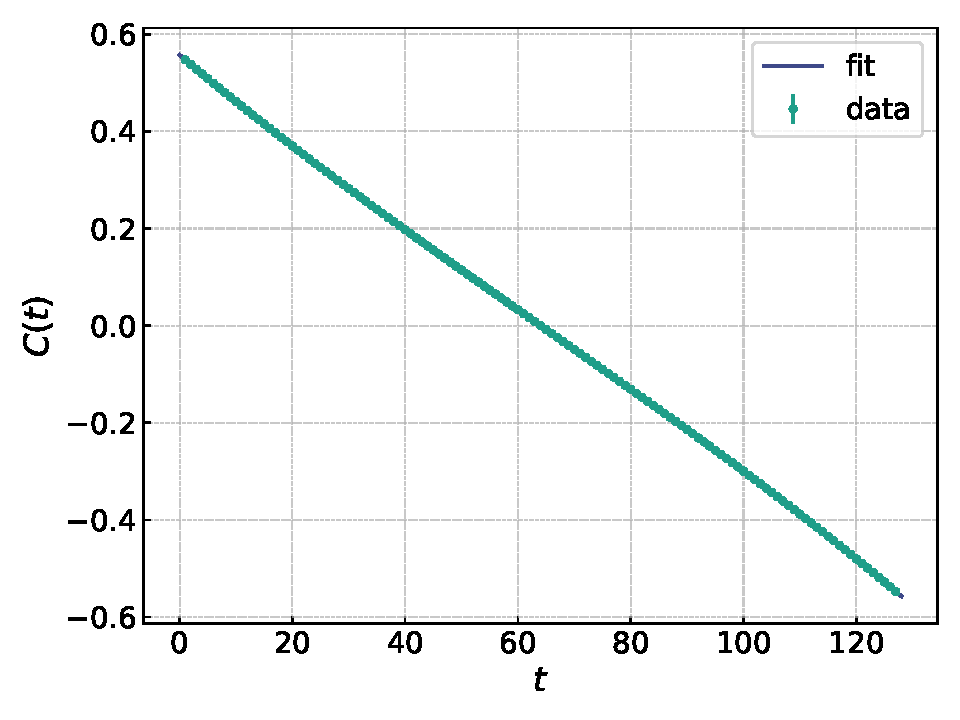
\includegraphics[width=1.05\textwidth]{figures/correlator/corrs_free/corr_small.pdf}
        \caption{$m_q = 0.01$}
    \end{subfigure}
    \hfill
    \begin{subfigure}[b]{0.48\textwidth}
        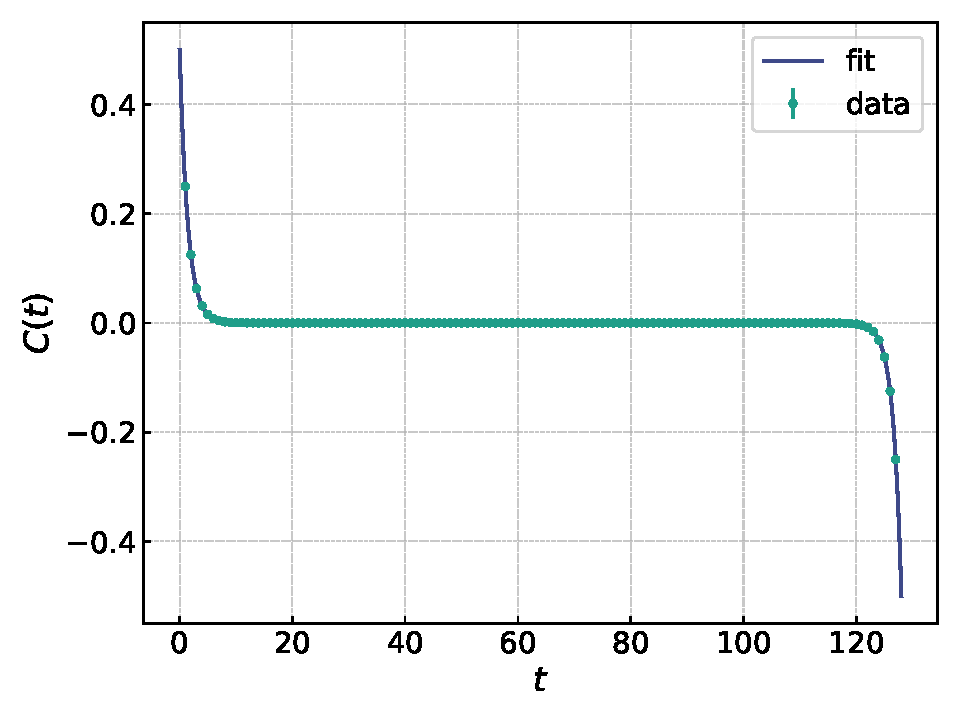
\includegraphics[width=1.05\textwidth]{figures/correlator/corrs_free/corr_big.pdf}
        \caption{$m_q = 1.0$}
    \end{subfigure}
    \\
    \vspace{10pt}
    \begin{subfigure}[b]{0.68\textwidth}
        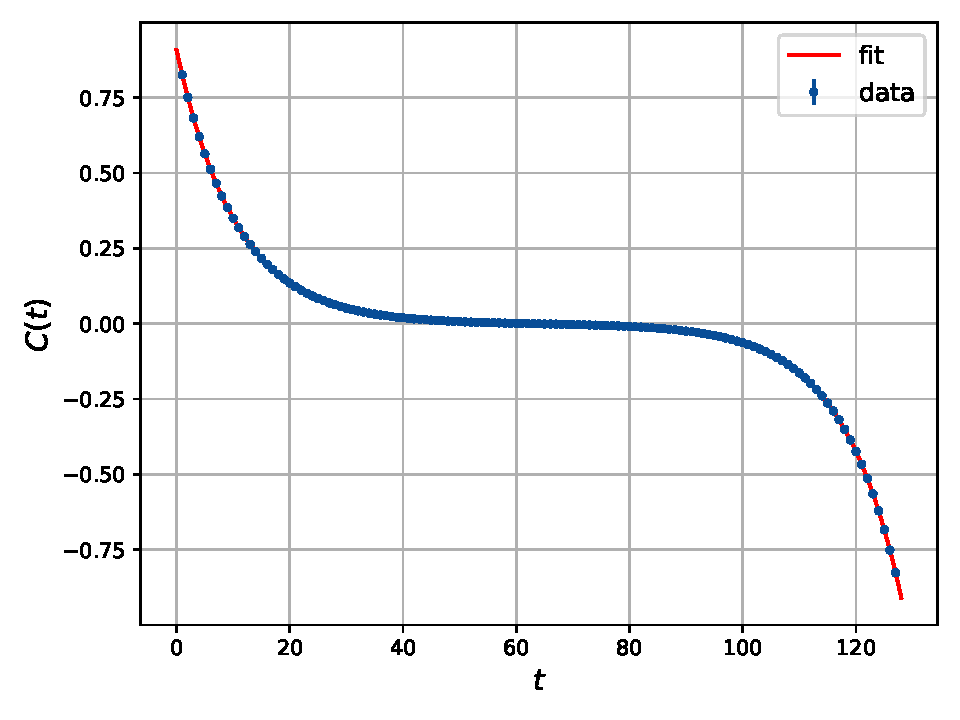
\includegraphics[width=1.05\textwidth]{figures/correlator/corrs_free/corr_medium.pdf}
        \caption{$m_q = 0.1$}        
    \end{subfigure}
    \caption[Fit of the correlator for free Wilson fermions.]{Fit of the fermionic correlator to \textcolor{red}{(eqref)}, for three different values of the bare quark mass.}
    \label{fig:fit_wilson}
\end{figure}
\textcolor{green}{The presence of a background field has the same effects on the correlator as a bare quark mass. In fact, if $\phi(x) = v$, one can simply redefine the bare mass as $M_q = m_q + g \, v$ and the properties of the fermionic correlator remain unchanged.}
\newpage

\section{Phase structure}
We want to start the analysis of the Yukawa theory by doing a parameters scan, in order to have a global picture of the phase diagram in the presence of Wilson fermions. For the remaining of this section, we set the value of the fermionic bare mass to $m_q = 1.0$.\\~\\
Figure \ref{fig:phase_diagram_g_m} reports a slice of the phase diagram in the $g-m_\phi^2$ plane. \\
For $g=0$, one reduces to the case of a O(1) scalar theory: for $m_\phi^2>0$ the systems lies in a symmetric state identified by $\expect{\phi} = 0$. 
As the mass goes to negative values, the scalar field gains a non-zero expectation value, signaling the spontaneous breaking of the O(1) symmetry. \\
When a finite Yukawa coupling is added, the finite bare quark mass and the Wilson term break chiral symmetry explicitly, resulting in a non-zero expectation value of the scalar field. \\
This is in good agreement with the qualitative description of the phase structure given in section \ref{sec:Yukawa_theory}.
\begin{figure}[htp]
    \centering
    \begin{subfigure}[b]{0.48\textwidth}
        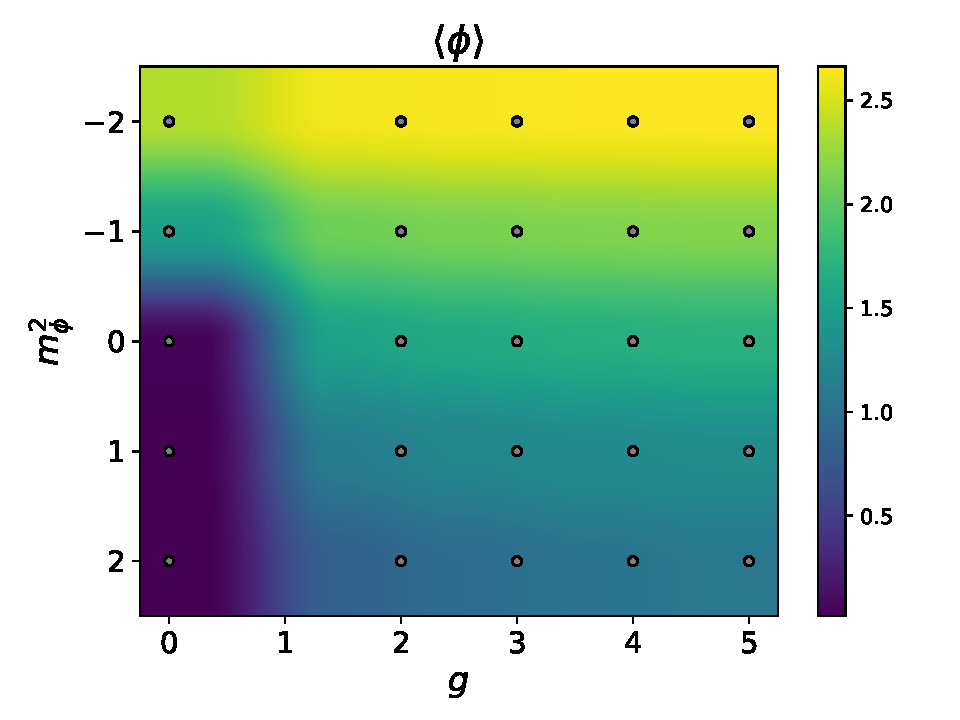
\includegraphics[width=\textwidth]{figures/phase_diagram/g-m/phase_diagram_phi.pdf}
    \end{subfigure}
    \begin{subfigure}[b]{0.48\textwidth}
        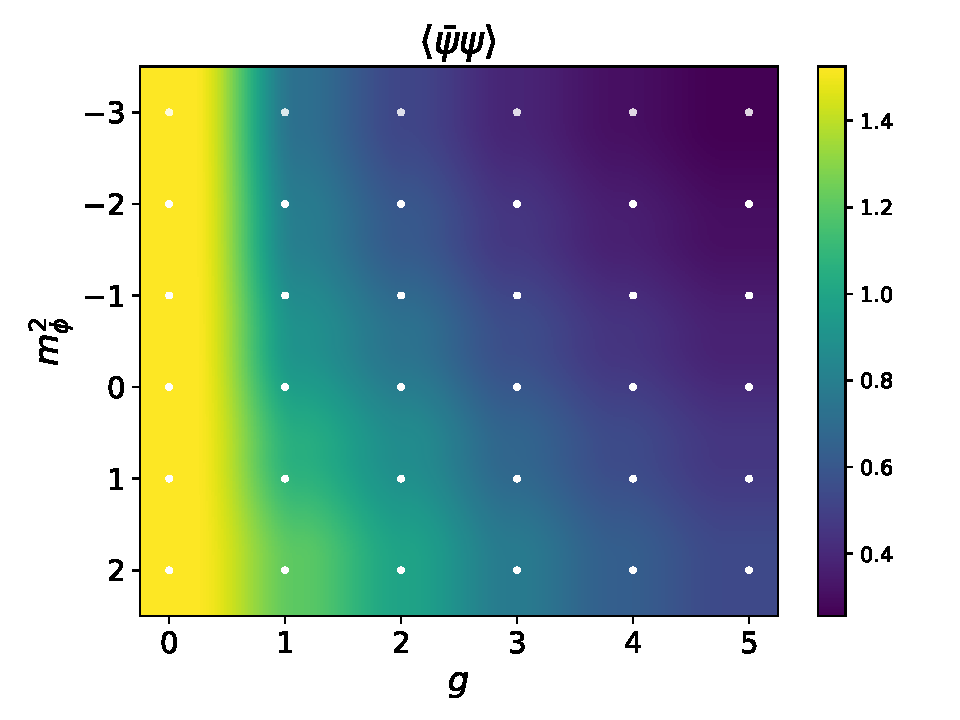
\includegraphics[width=\textwidth]{figures/phase_diagram/g-m/phase_diagram_cond.pdf}
    \end{subfigure}
    \begin{subfigure}[b]{0.48\textwidth}
        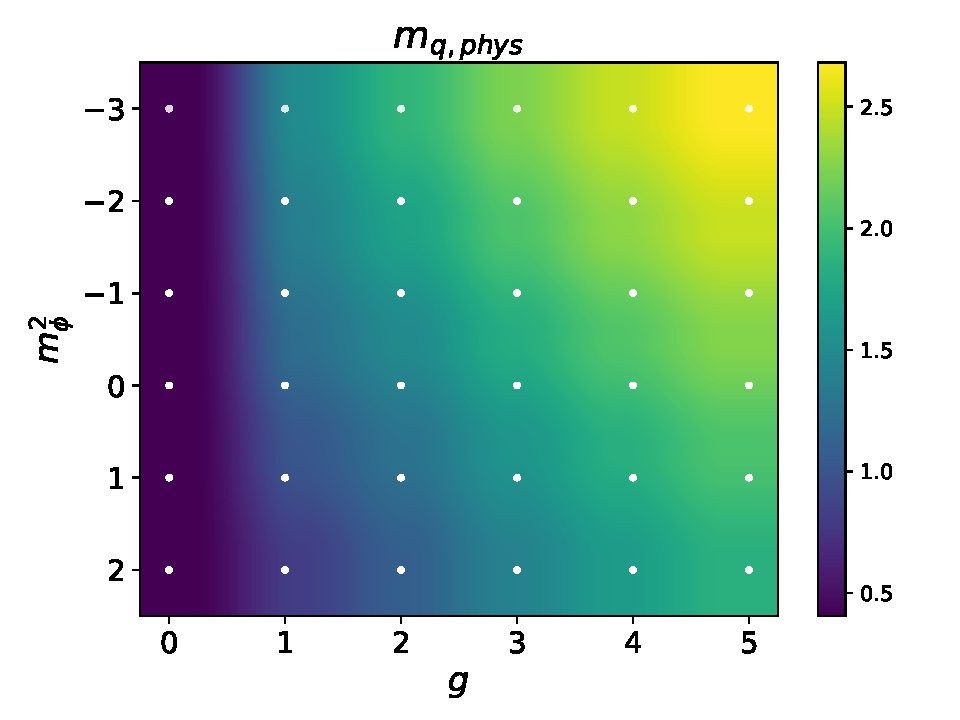
\includegraphics[width=\textwidth]{figures/phase_diagram/g-m/phase_diagram_mqphys.pdf}
    \end{subfigure}
    \begin{subfigure}[b]{0.48\textwidth}
        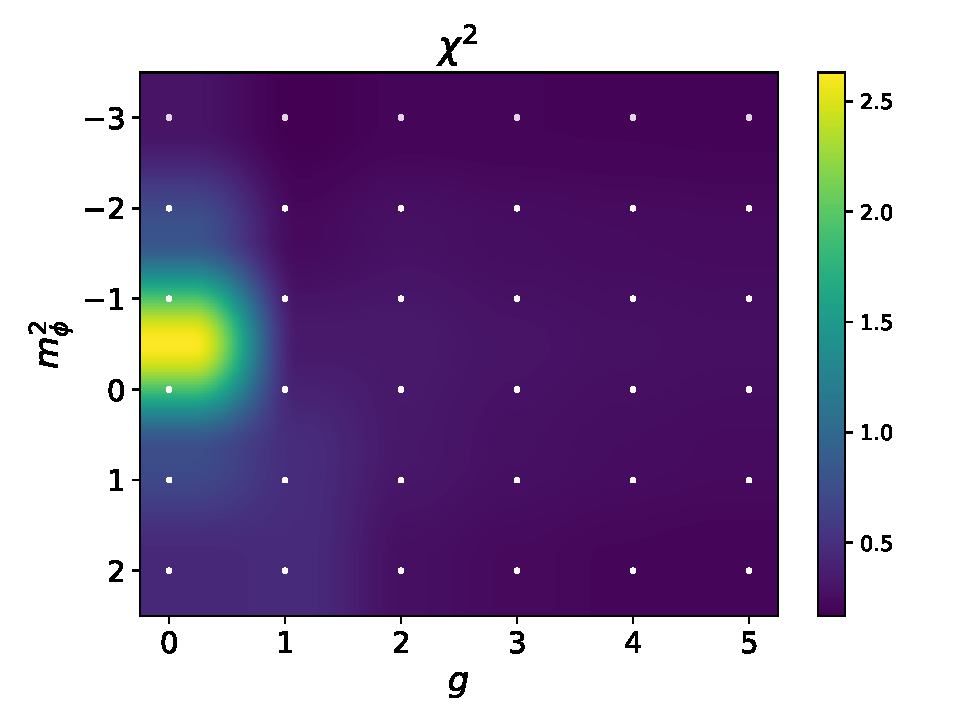
\includegraphics[width=\textwidth]{figures/phase_diagram/g-m/phase_diagram_chi2.pdf}
    \end{subfigure}
    \caption{Slice of the phase diagram at fixed $\lambda = 2.0$. \\ Lattice size $32 \times 32$, $N_\text{conf} \approx \mathcal{O}(5 \cdot 10^4)$.}
    \label{fig:phase_diagram_g_m}
\end{figure}\\
For finite $m_q$ and $g$ one cannot speak of a proper phase transition, as the symmetry is explicitly broken at the classical level. Thus, one still have a smooth crossover between the two phases. This fact is reflected in the plot of the magnetic susceptibility, which peaks around $m_\phi^2 = 0$ only for small values of $g$. \\
As explained in section \ref{sec:Yukawa_theory}, and shown in \textcolor{red}{where?}, the presence of a background scalar field can be interpreted as a bare quark mass. This is reflected in the plot of of $m_{q, \text{phys}}$ which resembles the one of $\expect{\phi}$, except for $g=0$, where the two theories are disconnected. \\
Finally, the chiral condensate, \dots \textcolor{red}{why the hell is is bigger for smaller g? I thought the bigger the condensate, the bigger the breaking.} \\~\\
Figure \ref{fig:phase_diagram_g_lam} reports the phase diagram in the $\lambda - g$ plane. The behavior can be understood qualitatively by means of classical arguments. 
For $g=0$, one expects a field magnetisation of order 
\begin{equation*}
    v = \sqrt{-\frac{6 m_\phi^2}{\lambda}}.
\end{equation*}
Hence, as $\lambda$ is increased, the expectation value of the field is reduced.
If $g \neq 0$, the fermion masses contributions increase the expectation value of the field, which in turns works as an additional bare quark mass, hence increasing $m_{q, \text{phys}}$. The behavior of the susceptibility is analogous to the previous case: only if $g=0$ one has a proper phase transition, reflected in the peak around $\lambda = 0, g = 0$.
\begin{figure}[htp]
    \centering
    \begin{subfigure}[b]{0.48\textwidth}
        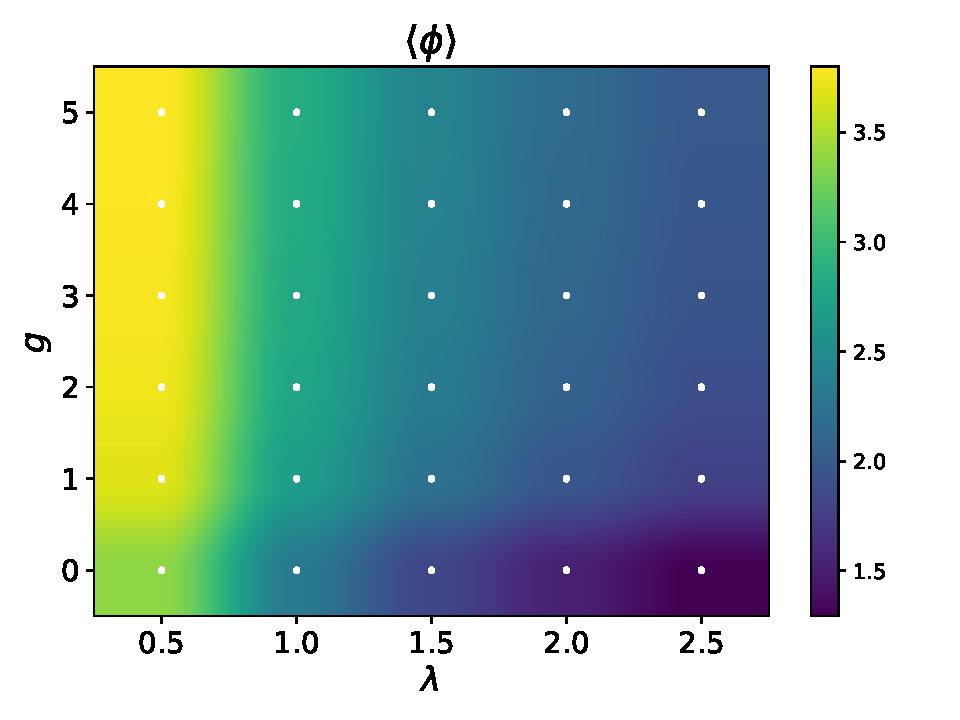
\includegraphics[width=\textwidth]{figures/phase_diagram/g-lam/phase_diagram_phi.pdf}
    \end{subfigure}
    \begin{subfigure}[b]{0.48\textwidth}
        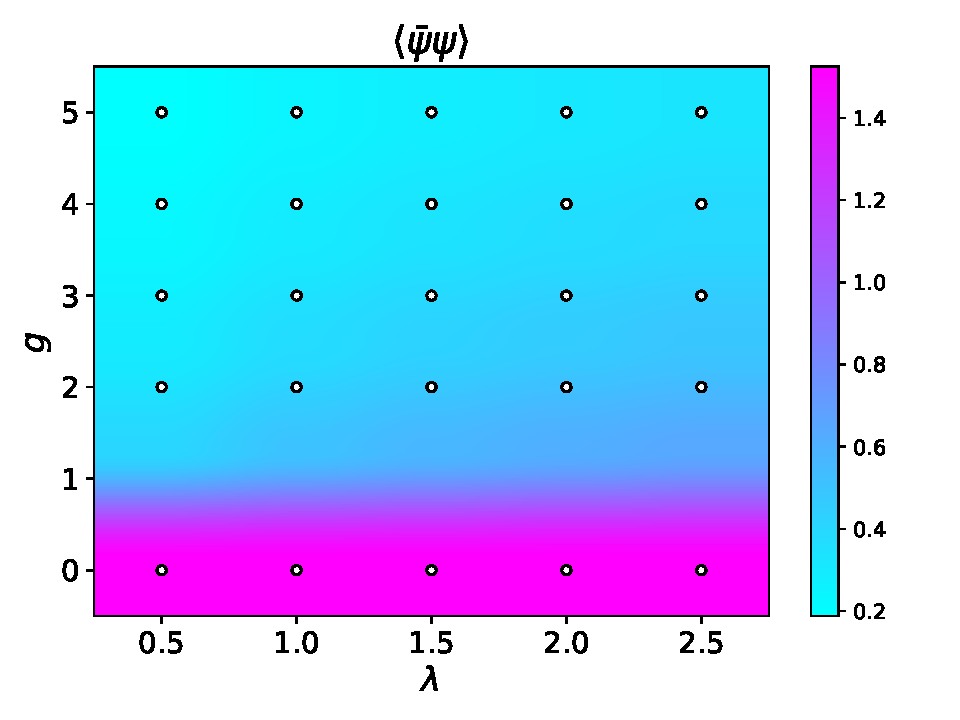
\includegraphics[width=\textwidth]{figures/phase_diagram/g-lam/phase_diagram_cond.pdf}
    \end{subfigure}
    \begin{subfigure}[b]{0.48\textwidth}
        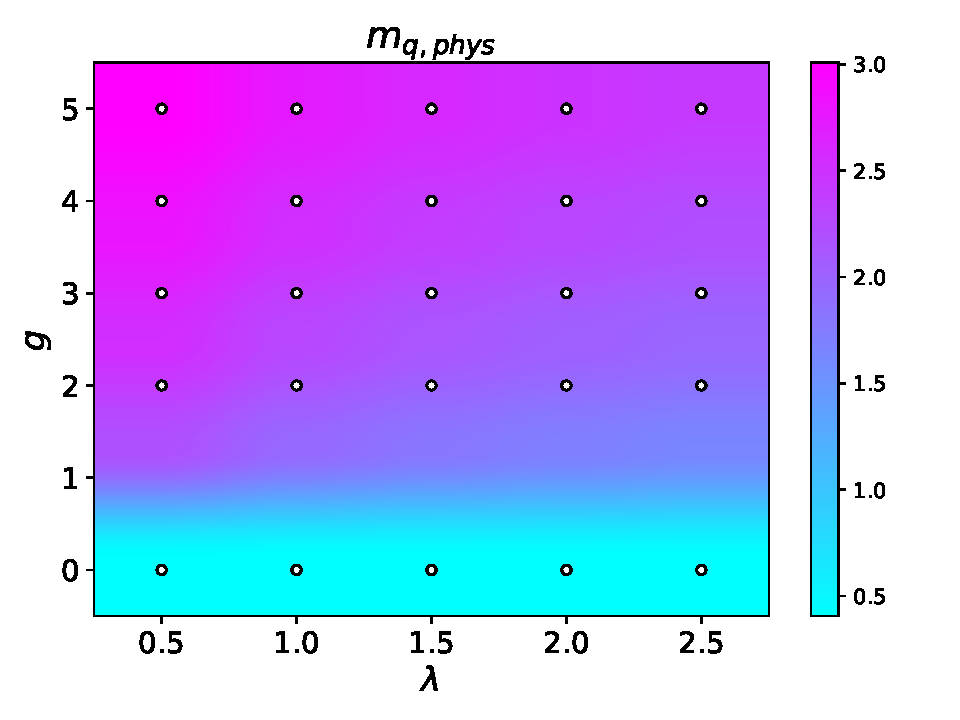
\includegraphics[width=\textwidth]{figures/phase_diagram/g-lam/phase_diagram_mqphys.pdf}
    \end{subfigure}
    \begin{subfigure}[b]{0.48\textwidth}
        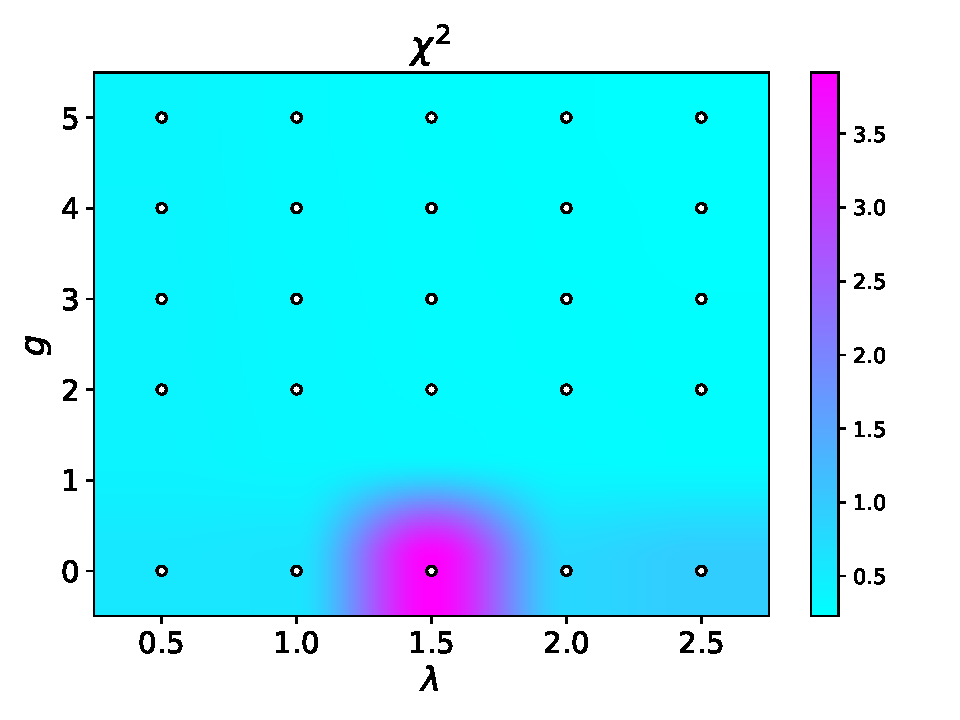
\includegraphics[width=\textwidth]{figures/phase_diagram/g-lam/phase_diagram_chi2.pdf}
    \end{subfigure}
    \caption{Slice of the phase diagram at fixed $m_\phi^2 = -1.0$. \\ Lattice size $32 \times 32$, $N_\text{conf} \approx \mathcal{O}(10^4)$.}
    \label{fig:phase_diagram_g_lam}
\end{figure}
\begin{figure}
    \centering
    \begin{subfigure}[b]{0.48\textwidth}
        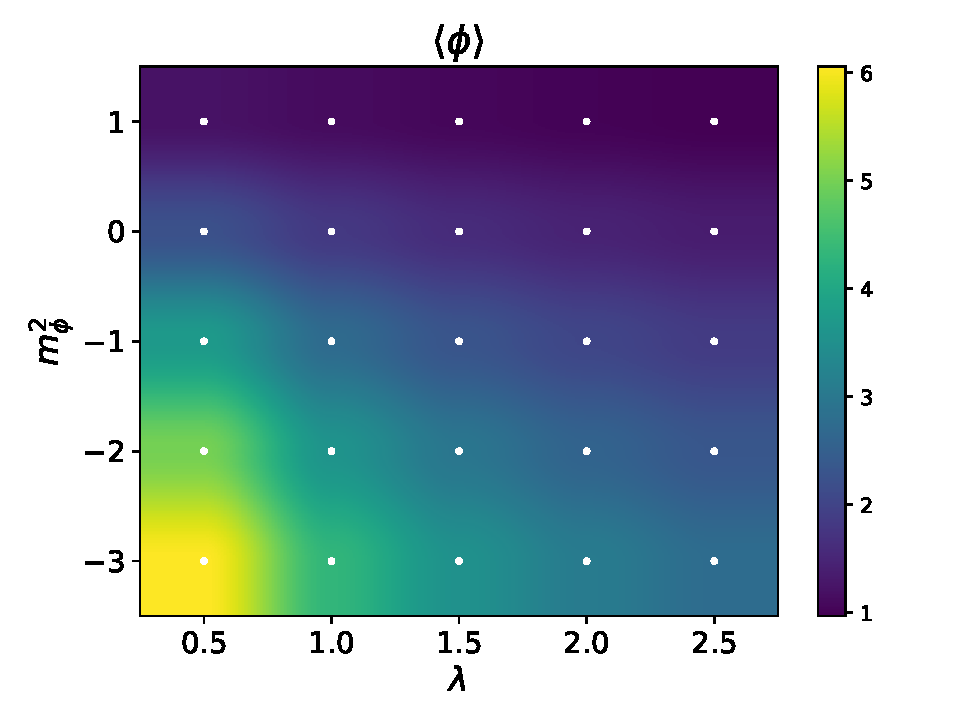
\includegraphics[width=\textwidth]{figures/phase_diagram/m-lam/phase_diagram_phi.pdf}
    \end{subfigure}
    \begin{subfigure}[b]{0.48\textwidth}
        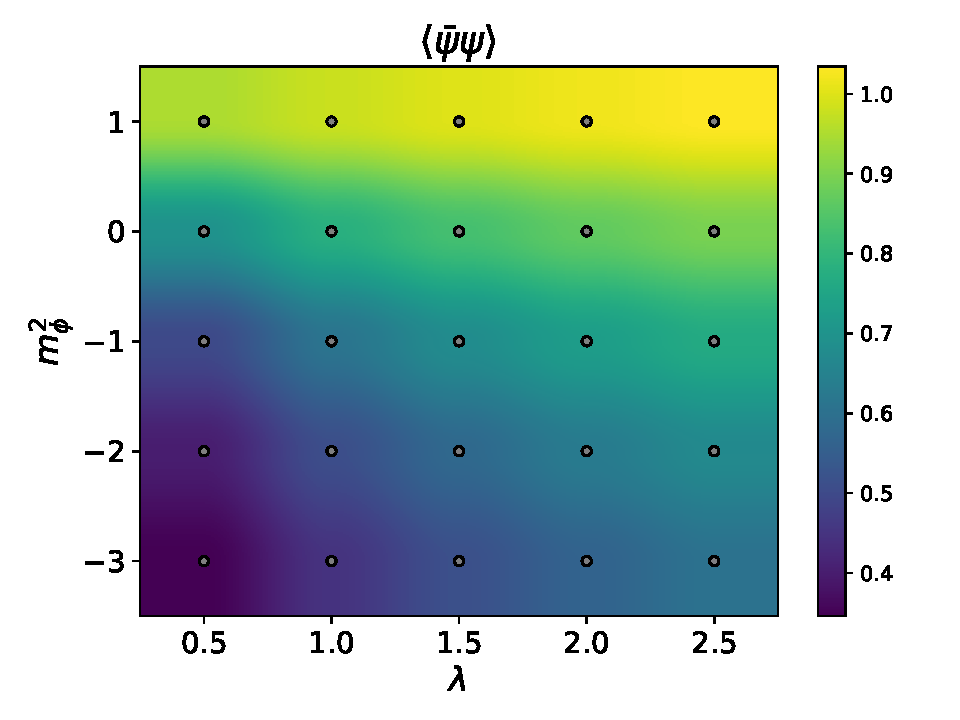
\includegraphics[width=\textwidth]{figures/phase_diagram/m-lam/phase_diagram_cond.pdf}
    \end{subfigure}
    \begin{subfigure}[b]{0.48\textwidth}
        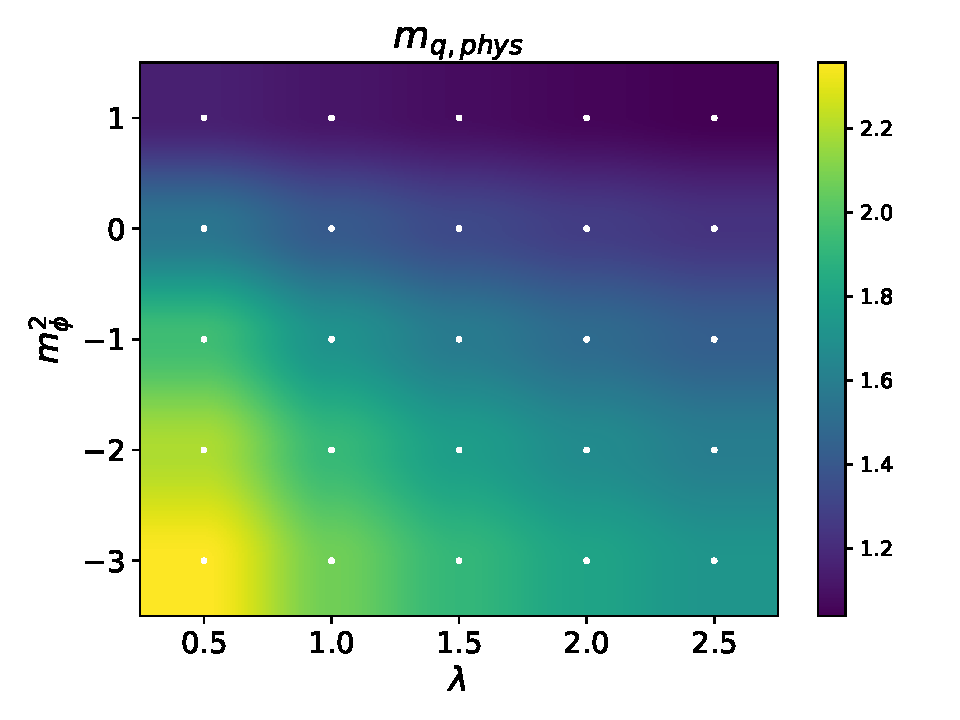
\includegraphics[width=\textwidth]{figures/phase_diagram/m-lam/phase_diagram_mqphys.pdf}
    \end{subfigure}
    \begin{subfigure}[b]{0.48\textwidth}
        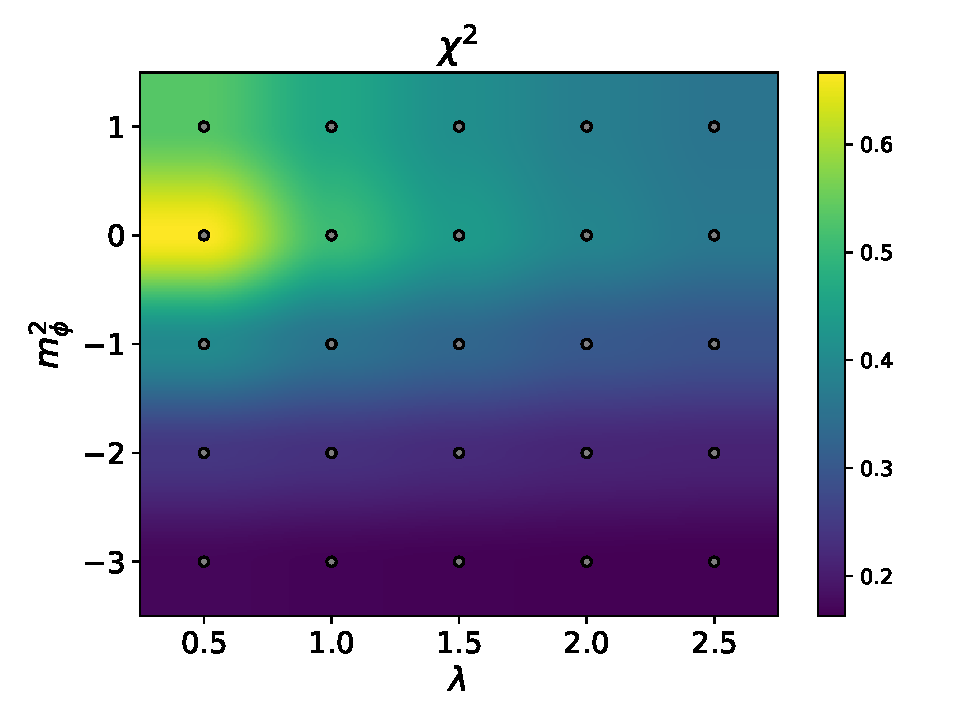
\includegraphics[width=\textwidth]{figures/phase_diagram/m-lam/phase_diagram_chi2.pdf}
    \end{subfigure}
    \caption{Slice of the phase diagram at fixed $g = 1.5$. \\ Lattice size $32 \times 32$, $N_\text{conf} \approx \mathcal{O}(10^4)$.}
    \label{fig:phase_diagram_m_lam}
\end{figure}\\

\chapter{Numerical results: coloured noise}
\label{chapt:results_coloured}

\section{Classical-to-quantum interpolation}

\label{sec:classical_to_quantum}

\begin{figure}[h]
    \centering
    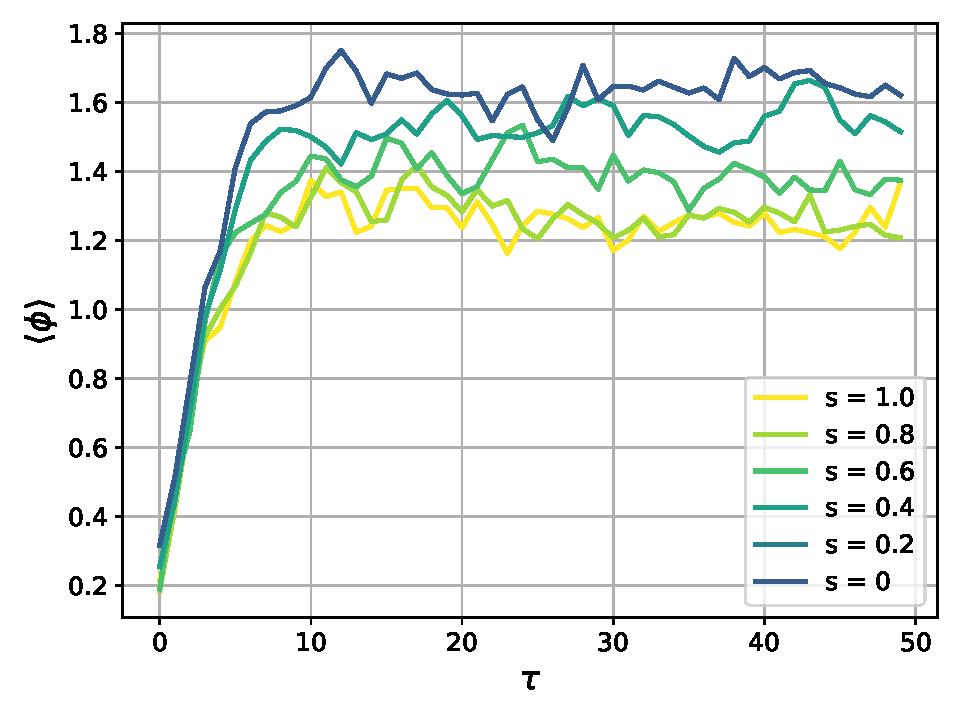
\includegraphics[width=0.8\textwidth]{figures/slide_broken/thermalisation.pdf}
    \caption[Thermalisation of the system for different values of the noise fraction $s$.]{Thermalisation of the system for different values of the noise fraction $s$. As noise is added, the equilibrium state of the system shifts accordingly. Coloured noise allows for a smooth interpolation between the fully classical and fully quantum picture.\\ Lattice size $32 \times 32, \ m_\phi^2=-1.0, \ \lambda=0.5, \ g=0.08, \ m_q = 0.5$.}
    \label{fig:thermalisation_different_noise_fracs}
\end{figure}

Let us start by analising the coloured noise field in the simulation and relevant properties that emerge from it. We consider the Yukawa model described by the continuum action \eqref{eq:full_action_continuum} and its discrete version \eqref{eq:discretised_action}, \eqref{eq:discretised_effective_action}.\\
The system is initialised in the same state for all the configurations on a $64 \times 64$ lattice. We consider a simulation with $s=1$ and then progressively lower the cutoff fraction $s$, keeping fixed all the quantities in the classical action. \\
Figure \ref{fig:thermalisation_different_noise_fracs} shows the system thermalisation for different values of $s$, namely the Langevin evolution from the initial state to equilibrium. The blue line corresponds to the case $s=0$, a classical simulation, while the brown line corresponds to the case $s=1$, the fully quantum case.  All the parameters settings are reported under the figure. \\
One can notice that as quantum modes are removed via coloured noise, the systems shifts its equilibrium point. \\~\\ 
In section \ref{sec:Yukawa_theory} it argued by using classical arguments that the magnetisation, chiral condensate and mass $m_{q, \text{phys}}$ are related via \eqref{eq:classical_EOM_full} and \eqref{eq:qualitative_relation_condensate_magnetisation_mass}. By looking at figure \ref{fig:interpolation_relation_phi_cond_mass} one can clearly see that 
\begin{equation*}
	\expect{\phi} \sim \expect{\bar\psi\psi} \sim m_q.
\end{equation*}
holds at all levels in the quantum theory. \\
This is an important result if one interprets it in the context of effective theories such as Gross-Neveu model, Quark-Meson model, NJL model, which are strictly related to our model as explained in section \textcolor{red}{???}. When one performs dynamical bosonisation via Hubbard Stratonovich transformation, the scalar field plays the role of a quark bilinear at all effects.
\begin{figure}[htp]
    \centering
    \begin{subfigure}[b]{0.48\textwidth}
        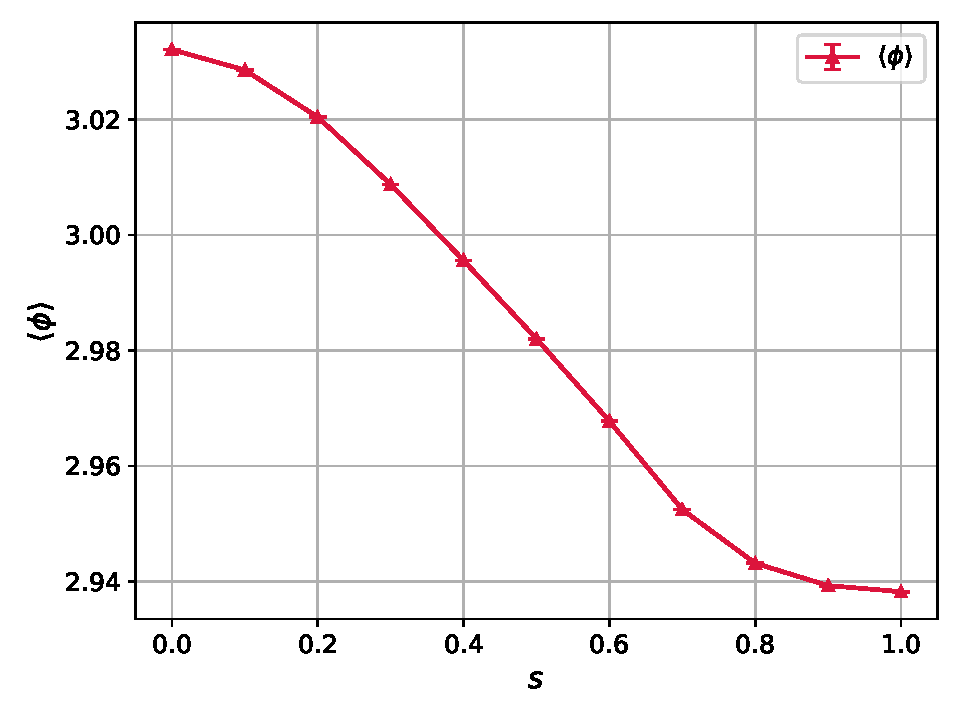
\includegraphics[width=1.0\textwidth]{figures/slide_broken/magnetisation.pdf}
    \end{subfigure}
    \begin{subfigure}[b]{0.48\textwidth}
        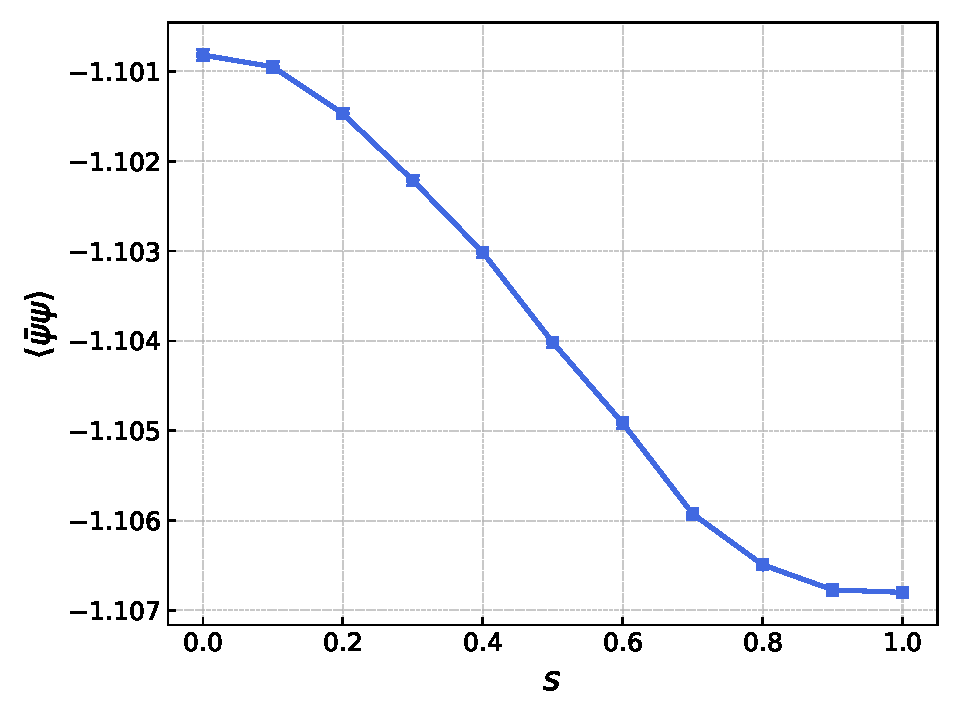
\includegraphics[width=1.0\textwidth]{figures/slide_broken/condensate.pdf}
    \end{subfigure}
    \begin{subfigure}[b]{0.48\textwidth}
        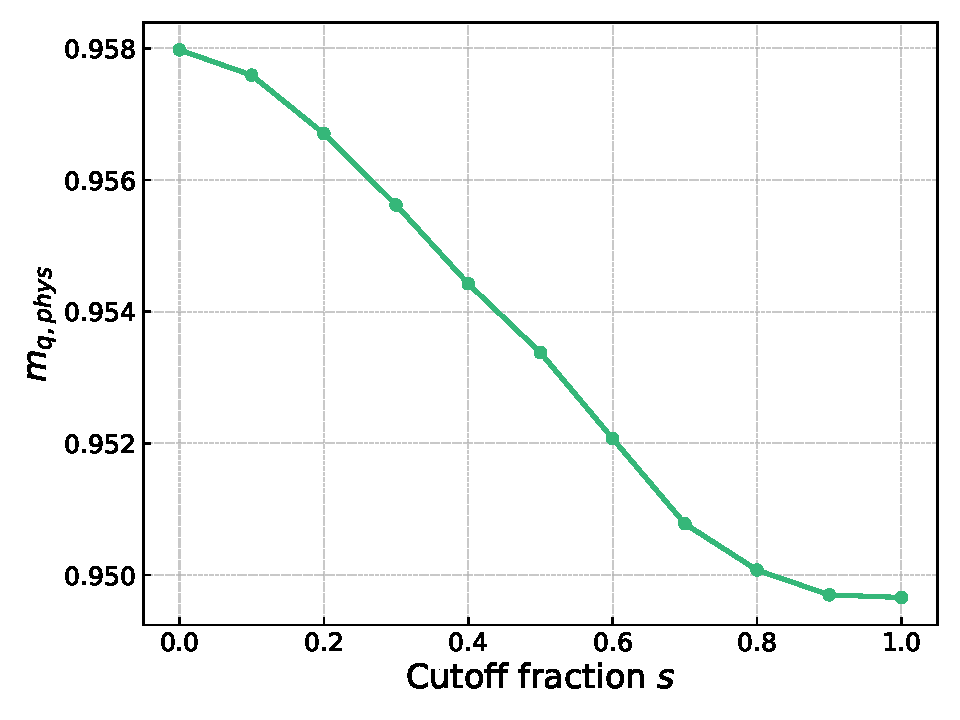
\includegraphics[width=1.0\textwidth]{figures/slide_broken/mass.pdf}
    \end{subfigure}
    \caption[Relation between magnetisation, condensate and mass]{\textcolor{red}{x label} Relation between magnetisation, chiral condensate and mass, which was motivated in section \ref{sec:Yukawa_theory}. \\ $m_\phi^2=-1.0, \ \lambda=0.7, g=0.2, \ m_q = 1.0$ \\ Lattice size $64 \times 64, \ N_\text{conf} \approx \mathcal{O}(5 \cdot 10^4)$.}
    \label{fig:interpolation_relation_phi_cond_mass}
\end{figure} \\
For $s=0$, the fields are restricted to the classical equations of motion \eqref{eq:classical_EOM_full}. As pointed out in section \ref{sec:Yukawa_theory}, in particular in equation \eqref{eq:background_field}, a background field $\phi(x) = v$ has the same behaviour on the system as a bare quark mass. We then compare the physical quark mass with the theoretical expression for free Wilson fermions \eqref{eq:analytical_wilson} using a shifted bare mass 
\begin{equation*}
	M_q = m_q + g \expect{\phi}
\end{equation*}
The comparison is reported in table \ref{tab:background_field}
\begin{table}[htp]
    \centering
    \begin{tabular}{cccccc}
        \toprule
        $m_q$ & $g$ & $\expect{\phi}$ & $M_q$ & $\log(1+M_q)$ & $m_\text{phys}$ \\
        \midrule
	$1.0$ & $0.2$ & 3.032082758 & 1.606416551
    & 0.957976309
    & 0.957976383 \\
        \bottomrule
    \end{tabular}
    \caption[Background field and quark mass]{The physical quark mass of the classical system is compared with the theoretical result for Wilson fermions, using the shifted bare mass $M_q = m_q + g \left\langle\phi\right\rangle$. This shows that a background scalar field can be interpreted as a bare quark mass.}
    \label{tab:background_field}
\end{table}

\newpage


\section{Chiral fermions and noise-induced chiral phase transition}
\label{sec:chiral_PT}
\textcolor{red}{comment on the configurations}
As explained in section \ref{sec:Yukawa_theory}, chiral symmetry can be broken, in the continumm theory, either explicitly via the introduction of a finite bare quark mass, or spontaneously if the field gains a non-zero expectation value.\\
Moreoveor, in the discrete formulation, the introduction of the Wilson term contributes to the explicit breaking of chiral symmetry, as shown in appendix \ref{chap:AppendixB}. This, in particular, means that chiral symmetry is explicitly broken also for $m_q \to 0$. Because of this, one needs a new definition of the bare mass $M_q$, which takes into account the Wilson term contribution, such that chiral symmetry is restored in the limit $M_q \to 0$. \\
In a lattice study of a theory suchs as  two-flavours QCD, what one typically does \cite{rothe_LGT,gattringer_LQCD} is the following: the spontaneous breaking of chiral symmetry generates three goldstone massless bosons, the pions. If the bare quark mass is zero, the physical mass of the pions has to be zero, as a consequence of Goldstone's theorem \cite{goldstone}. Hence one can measure the pions mass and find a value $m_q^*$ such that when $m_q \to m_q^*$ one has $M_\pi \to 0$. \\
This approach is not feasible in our theory, since it is described by a discrete chiral symmetry. \\
In the literature, one can find proposals for the definition of a bare quark mass for similar theories \cite{Iwasaki:1994gq,MAIANI1986265}. Thus such approaches are not followed here, both because of time reasons, but also because it is not our purpose to match any physical results, but rather investigate properties of the coloured noise technique. Hence, here we just consider na\"ive fermions and the chiral limit is reached for $m_q \to 0$. Thus, one has to keep in mind that due to the fermion doubling, this represents a theory with $2N_f = 4$ physical degenerate quarks. \\~\\
\begin{figure}[h]
    \centering
    \captionsetup[subfigure]{justification=centering}
    \begin{subfigure}[t]{0.48\textwidth}
        \centering
        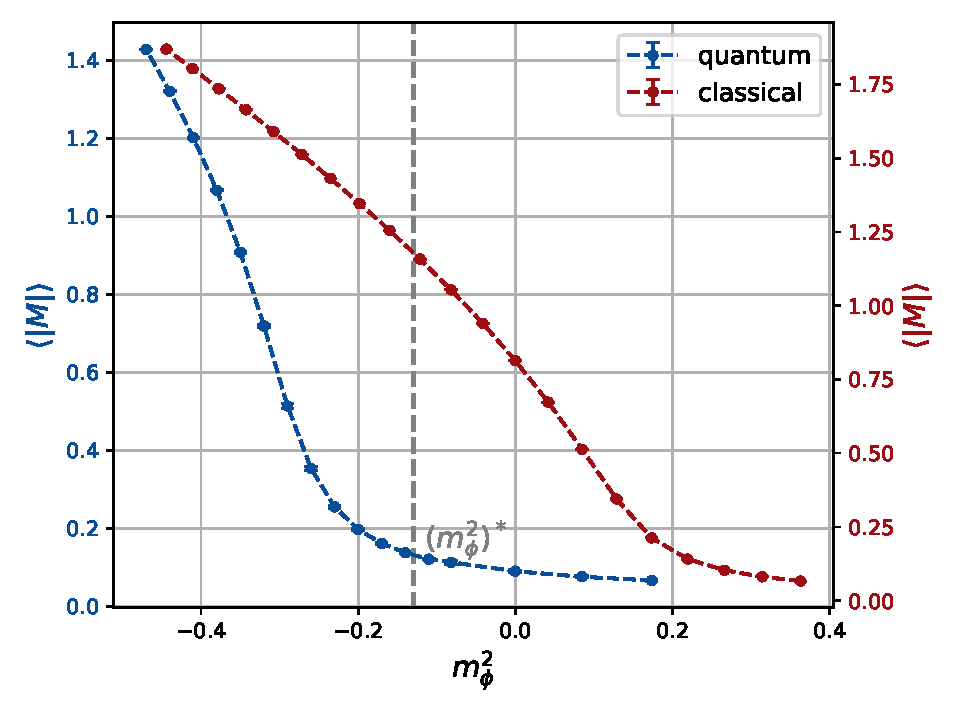
\includegraphics[width=1.05\textwidth]{figures/chiral_PT/mass_scan/magnetisation.pdf}
    \end{subfigure}
    \hfill
    \begin{subfigure}[t]{0.48\textwidth}
        \centering
        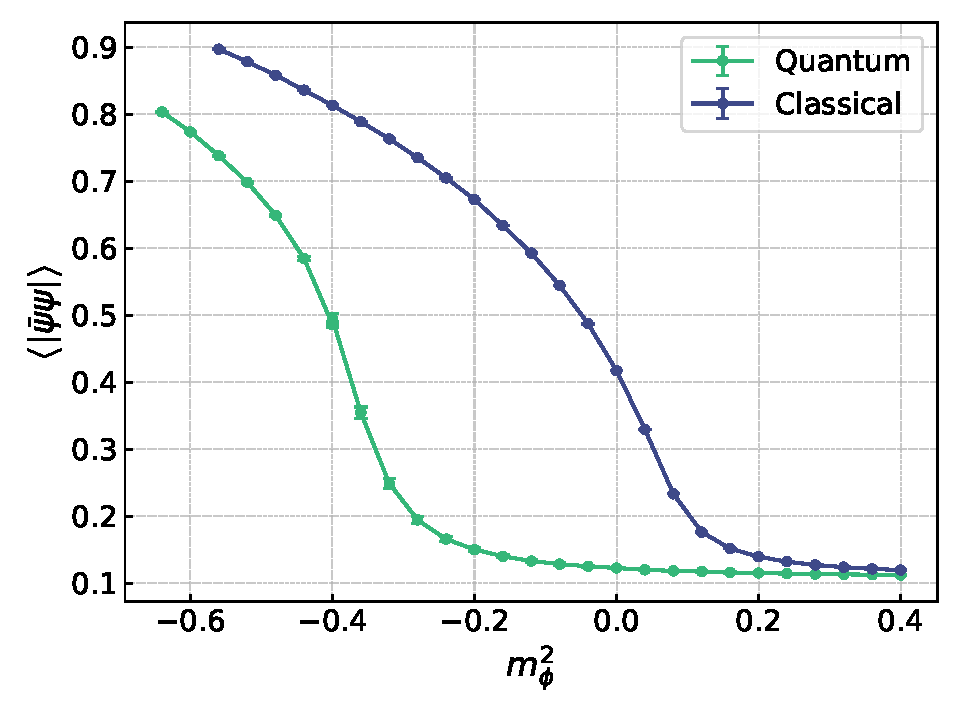
\includegraphics[width=1.05\textwidth]{figures/chiral_PT/mass_scan/condensate.pdf}
    \end{subfigure}
    \caption[Mass scan of the quantum and classical theories]{Mass scan of the quantum and classical theories. The dashed gray line indicates a value $m_\phi^{2, \,*}$, where the classical and quantum systems lie in two different phases.}
    \label{fig:scans_classical_quantum}
\end{figure} 
In figure \ref{fig:scans_classical_quantum}, the (absolute) magnetisation and the chiral condensate are studied as a function of the bosonic mass squared, both in the fully quantum and fully classical theory. One can notice that the classical system undergoes a phase transition at values of $m_\phi^2$ bigger than the quantum counterpart. Note that as the bare quark mass is small but finite, this is not a proper phase transition and the latter will be, eventually, reached in the limit $m_q \to 0$. We then pick a value $m_\phi^{2 \, *} = -0.123$ which is represented by a gray line in figure \ref{fig:scans_classical_quantum}.
Using coloured noise, we then interpolate between the classical and quantum picture for different values of the quark mass, namely $m_q = 10^{-2}, 5 \cdot 10^{-3}, 10^{-3}$.
\begin{figure}[h!]
\centering
\begin{minipage}{0.45\textwidth}	
	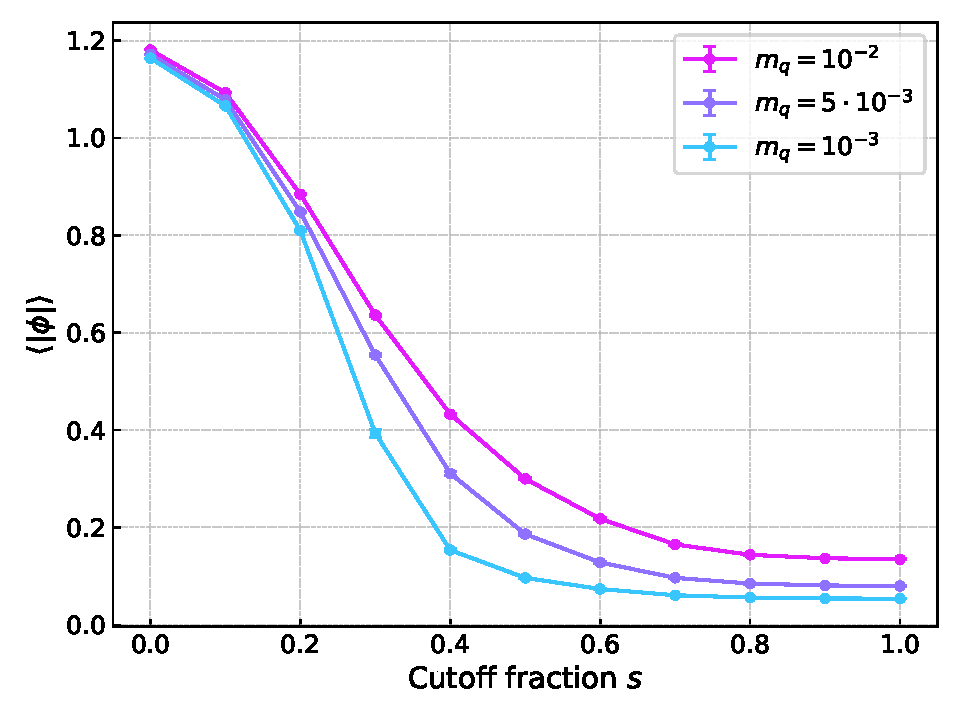
\includegraphics[scale=0.48]{figures/chiral_PT/magnetisation.pdf}
\end{minipage}
\hfill
\begin{minipage}{0.45\textwidth}	
	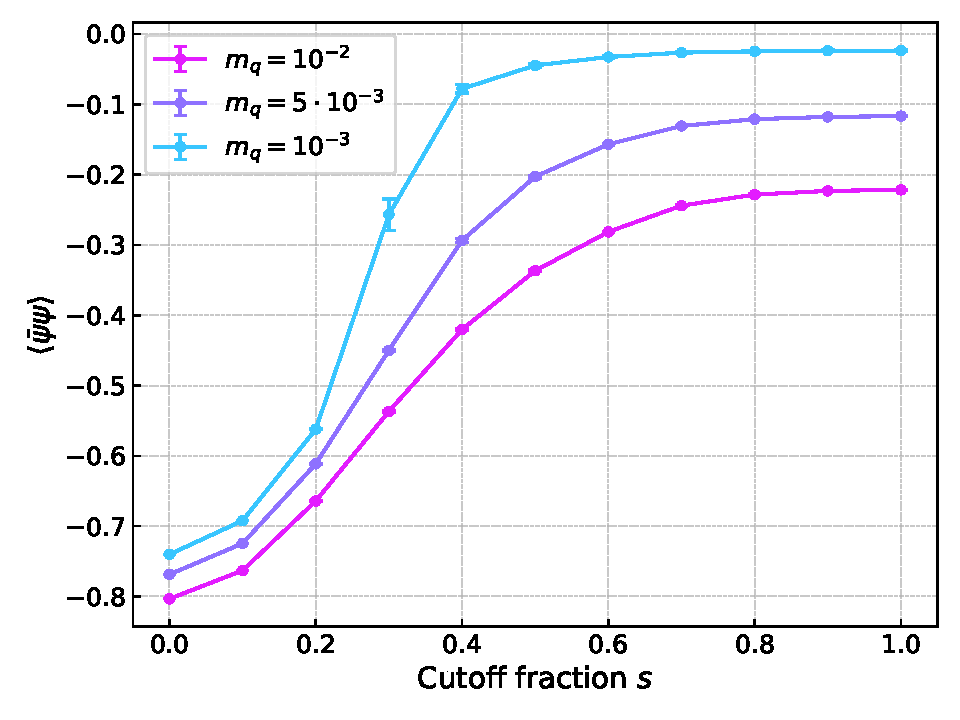
\includegraphics[scale=0.48]{figures/chiral_PT/condensate.pdf}
\end{minipage}
\begin{minipage}{0.45\textwidth}	
	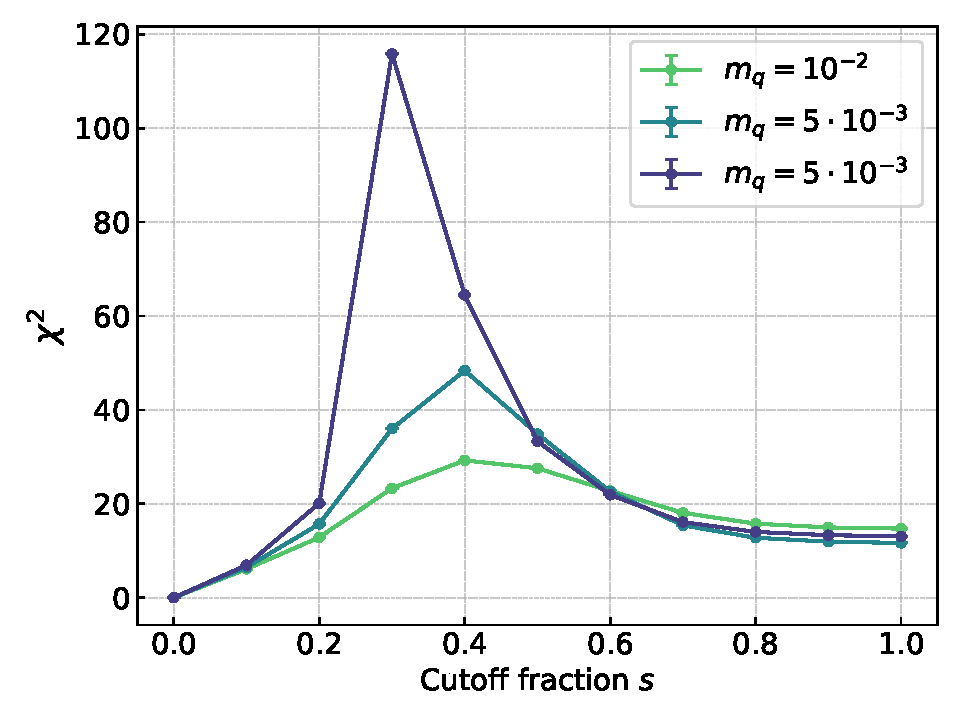
\includegraphics[scale=0.48]{figures/chiral_PT/chi2.pdf}
\end{minipage}
\hfill
\begin{minipage}{0.45\textwidth}
	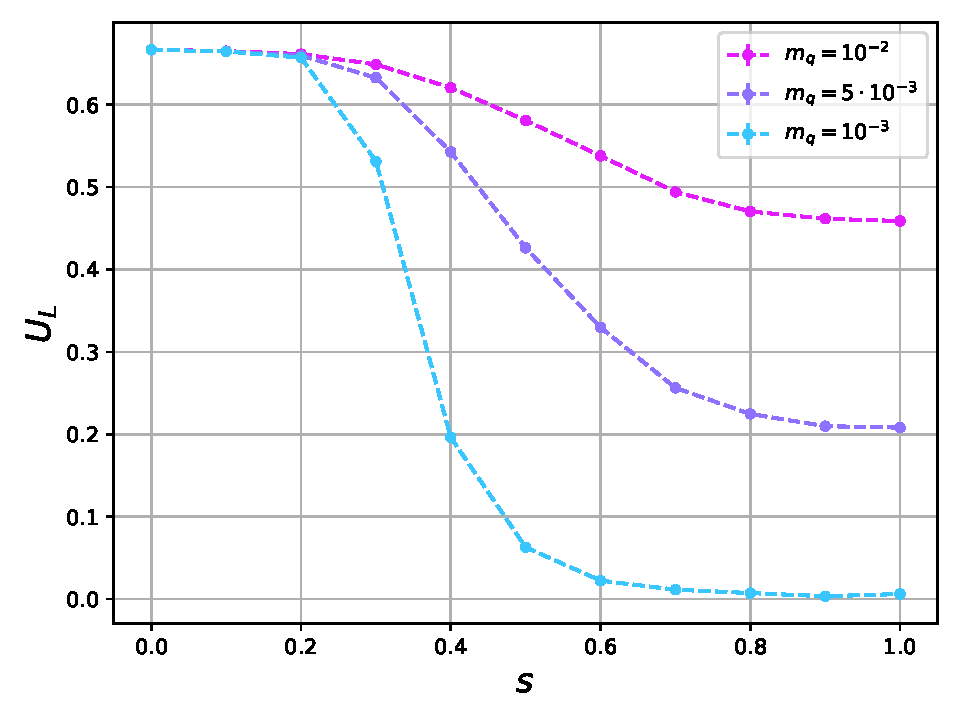
\includegraphics[scale=0.48]{figures/chiral_PT/binder.pdf}
\end{minipage}
\hfill
\caption{$m_\phi^2=-0.123, \ \lambda=1.951, g=0.08,$ \\ Lattice size $64 \times 64, \ N_\text{conf} \approx \mathcal{O}(5 \cdot 10^4)$}
\label{fig:chiral:symmetry_breaking}
\end{figure}\\

One can clearly see in figure \ref{fig:chiral:symmetry_breaking} that as the quark  mass is lowered the difference between the two phases gets sharper, indicating a phase transition. 
This is especially highligthed in the increasing peak of the magnetic susceptibility, and by the Binder parameters, which is supposed to assume the vlaue $U_L = 0$ in the symmetric phase, and $U_L=2/3$ in the broken phase.

\newpage
\textcolor{red}{EMPTY}
\newpage

\section{Cooling with coloured noise}
Let us now consider one of the main applications of coloured noise, namely the cooling technique. \\
We first set up a white noise simulation $s=1$, and then progressively lower $s$. The lowering of the cutoff is compensated by a change in the couplings, as explained in section \ref{sec:lattice_with_coloured_noise}. 
We study the behavior of the system both as a function of the bosonic mass squared $m_\phi^2$ and the yukawa coupling $g$. 
A summary of the parameters choice for both the experiments is reported in tables \ref{tab:params_cooling} and \ref{tab:params_cooling_yukawa}. \\
\begin{table}[htp]
    \centering
    \begin{tabular}{cccccccc}
        \toprule
        $s$ & $N_t$ & $N_x$ & $m_\phi^2$ & $\lambda$ & $g$ & $m_q$& $K_\psi$ \\
        \midrule 
        1 & 16 & 16 & $m_\phi^2$ & 0.4 & 0.3 & $0.5$ & $K_\psi$ \\
        1/2 & 32 & 32 & $m_\phi^2/4$ & 0.1 & 0.3 & $0.5$ & $K_\psi/4$ \\
        1/4 & 64 & 64 & $m_\phi^2/16$ & 0.025 & 0.3 & $0.5$ & $K_\psi/16$ \\
        1/8 & 128 & 128 & $m_\phi^2/64$ & 0.00625 & 0.3 & $0.5$ & $K_\psi/64$ \\
        \bottomrule
    \end{tabular}
    \caption[Parameter settings in the cooling procedure for the Bosonic mass squared scan]{Parameter settings in the cooling procedure for the bosonic mass squared scan. Each coupling in the bosonic action is rescaled according to its canonical dimension, while the fermionic sector rescaling is implemented directly at the drift level, as detailed in section \ref{sec:lattice_with_coloured_noise}}.
    \label{tab:params_cooling}
\end{table}
\begin{table}[htp]
    \centering
    \begin{tabular}{cccccccc}
        \toprule
        $s$ & $N_t$ & $N_x$ & $m_\phi^2$ & $\lambda$ & $g$ & $m_q$& $K_\psi$ \\
        \midrule 
        1 & 16 & 16 & $0.5$ & 0.7 & g & $1.0$ & $K_\psi$ \\
        1/2 & 32 & 32 & $0.125$ & 0.175 & g & $1.0$ & $K_\psi/4$ \\
        1/4 & 64 & 64 & $0.0625$ & 0.04375 & g & $1.0$ & $K_\psi/16$ \\
        1/8 & 128 & 128 & $0.03125$ & 0.001094 & g & $1.0$ & $K_\psi/64$ \\
        \bottomrule
    \end{tabular}
    \caption[Parameter settings in the cooling procedure for the Yukawa coupling scan.]{Parameters setting in the cooling procedure for the Yukawa coupling scan. Each coupling in the bosonic action is rescaled according to its canonical dimension, while the fermionic sector rescaling is implemented directly at the drift level, as detailed in section \ref{sec:lattice_with_coloured_noise}}.
    \label{tab:params_cooling_yukawa}
\end{table}
Figure \ref{fig:cooling_M_psibarpsi_chi2} reports the magnetisation, its susceptibility and the chiral condensate as a function of the bare scalar mass squared $m_\phi^2$, while figure \ref{fig:cooling_M_psibarpsi} reports the investigation as a function of the Yukawa coupling. \\
One can clearly see that there is a general good agreement for the first three block-spin transformations.
\begin{figure}[hbp]
    \centering
    \begin{subfigure}[b]{0.48\textwidth}
        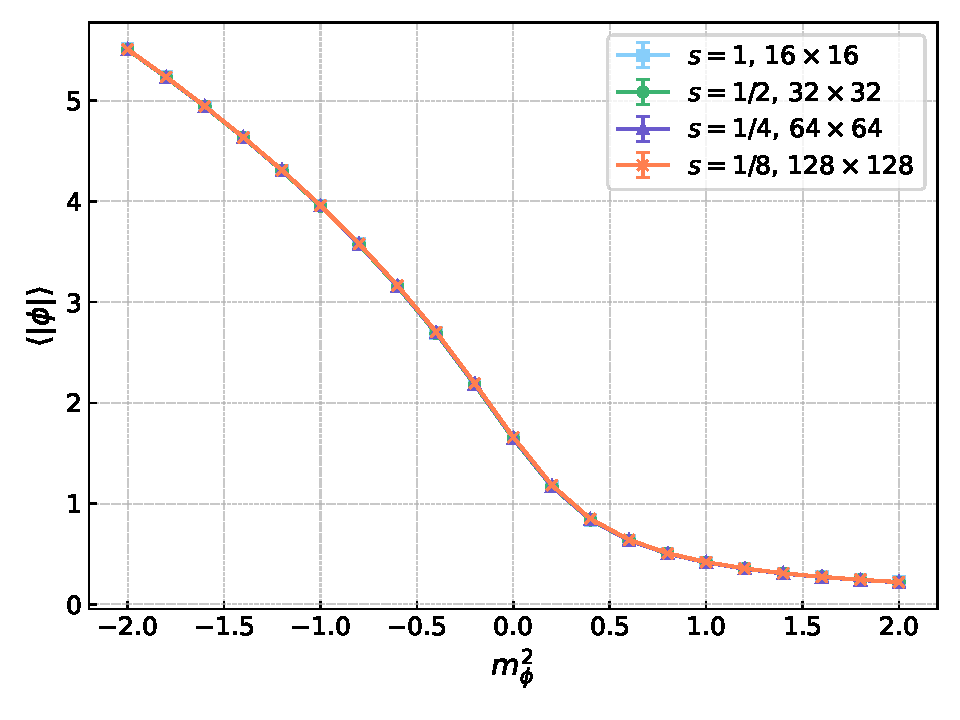
\includegraphics[width=1.05\textwidth]{figures/cooling/mass_scan/magnetisation.pdf}
    \end{subfigure}
    \hfill
    \begin{subfigure}[b]{0.48\textwidth}
        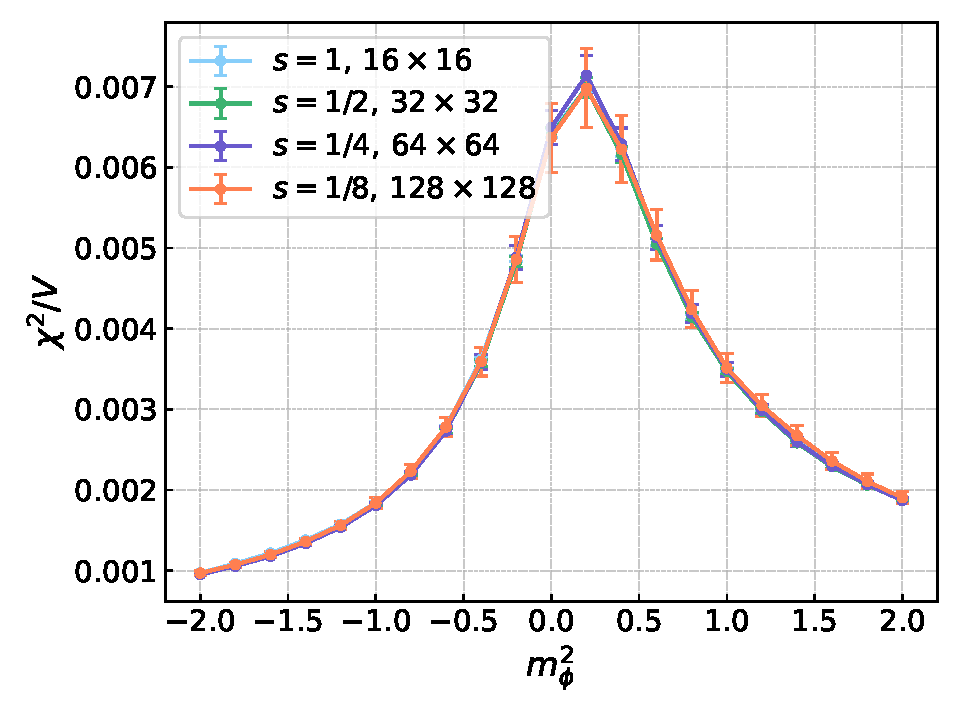
\includegraphics[width=1.05\textwidth]{figures/cooling/mass_scan/susceptibility.pdf}
    \end{subfigure}
    \begin{subfigure}[b]{0.48\textwidth}
        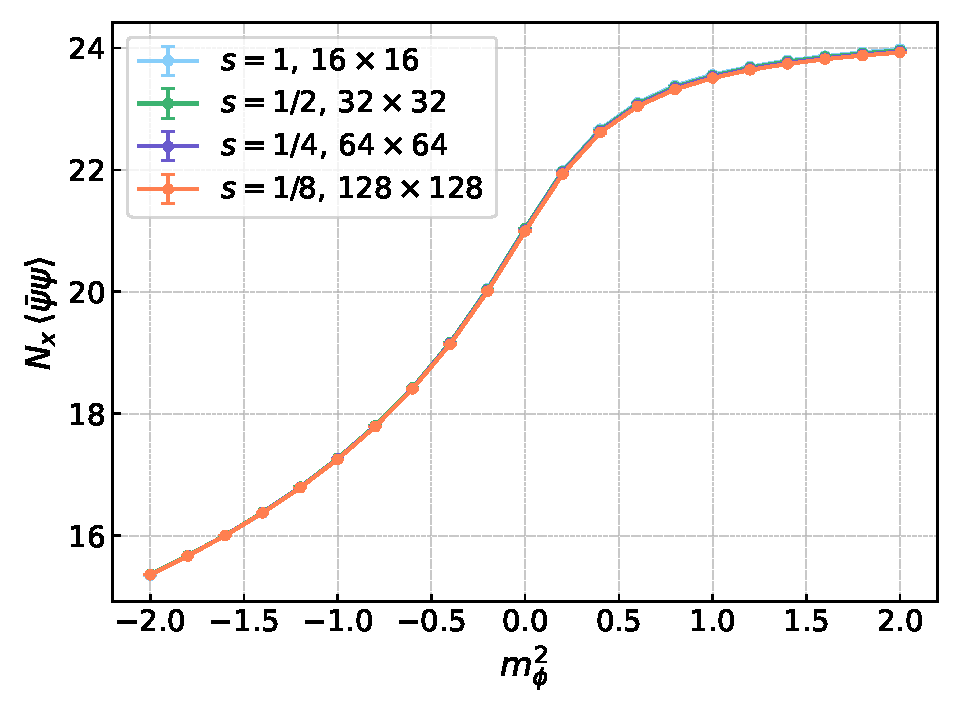
\includegraphics[width=1.05\textwidth]{figures/cooling/mass_scan/condensate.pdf}
    \end{subfigure}
    \caption[Cooling stochastic quantisation: fields as a function of the bosonic mass squared.]{Cooling via coloured noise. The absolute magnetisation, its susceptibility and the chiral condensate are compared after performing block-spins transformations as a function of the bosonic mass squared. \\ $N_\text{conf} \approx \mathcal{O}(5 \cdot 10^4)$. The other parameters are reported in table \ref{tab:params_cooling}}
    \label{fig:cooling_M_psibarpsi_chi2}
\end{figure}
\begin{figure}[hbp]
    \centering
    \begin{subfigure}[b]{0.48\textwidth}
        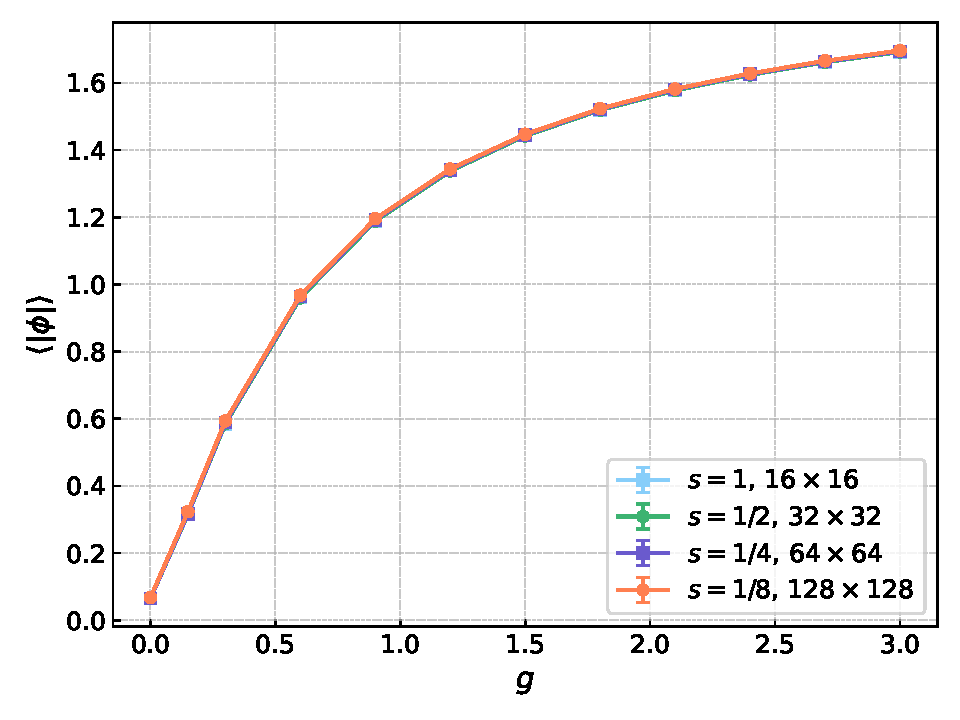
\includegraphics[width=1.05\textwidth]{figures/cooling/yukawa_scan/magnetisation.pdf}
    \end{subfigure}
    \hfill
    \begin{subfigure}[b]{0.48\textwidth}
        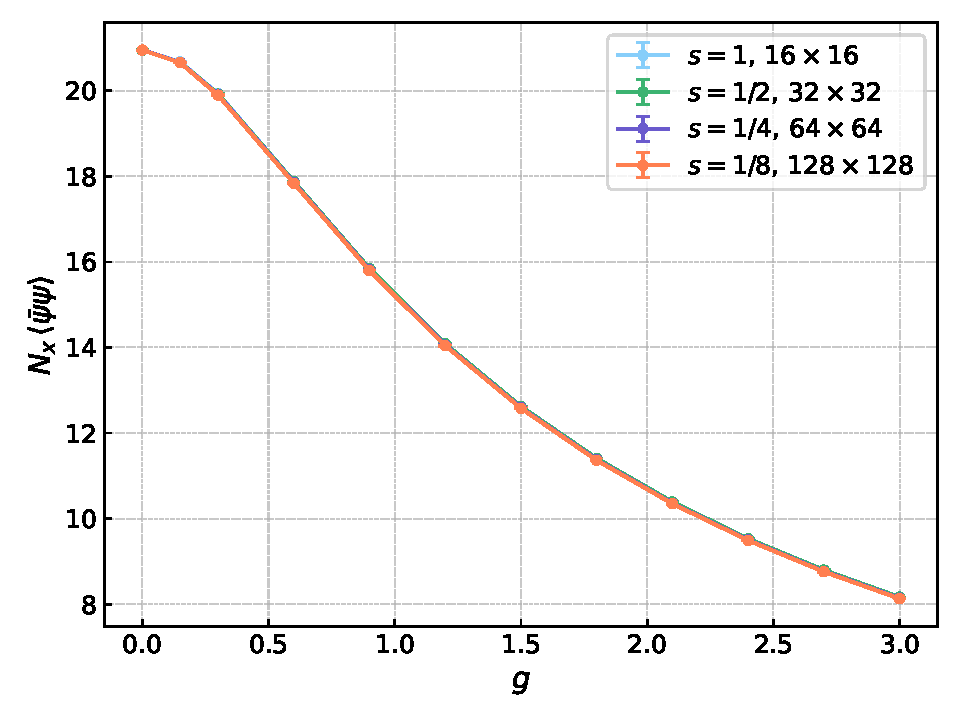
\includegraphics[width=1.05\textwidth]{figures/cooling/yukawa_scan/condensate.pdf}
    \end{subfigure}
    \caption[Cooling stochastic quantisation: fields as a function of the Yukawa coupling.]{Cooling via coloured noise. The absolute magnetisation and the chiral condensate are compared after performing block-spins transformations as a function of the Yukawa coupling. \\ $N_\text{conf} \approx \mathcal{O}(5 \cdot 10^4)$. The other parameters are reported in table \ref{tab:params_cooling_yukawa}.}
    \label{fig:cooling_M_psibarpsi}
\end{figure}\\
\newpage
The most relevant observables are the magnetisation and the chiral condensate, since they are the order parameters of the theory. We therefore want to provide a more detailed comparison of the performance of the procedure. To this end we define the relative errors
\begin{equation}
    \begin{aligned}
        \epsilon_\phi(s) &= \frac{\expect{|M|}_{s} - \expect{|M|}}{\expect{|M|}}, \\
        \epsilon_\psi(s) &= \frac{\expect{|\bar\psi \, \psi|}_{s} - \expect{|\bar\psi \, \psi||}}{\expect{|\bar\psi \, \psi||}}.
    \end{aligned}
    \label{eq:cooling_relative_deviation}
\end{equation}
The deviation quantified by such parameters is reported in figures \ref{fig:cooling_deviation} and \ref{fig:cooling_deviation_yukawa}.
\begin{figure}[htp]
    \centering
    \begin{subfigure}[b]{0.48\textwidth}
        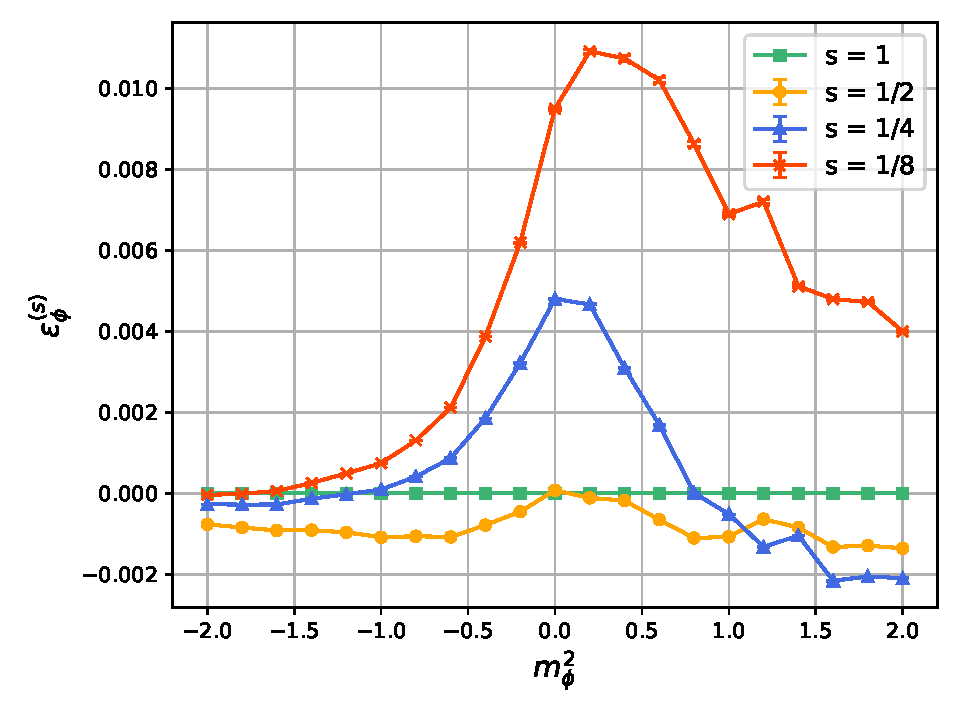
\includegraphics[width=1.0\textwidth]{figures/cooling/mass_scan/deviation.pdf}
        \caption{Absolute magnetisation}
    \end{subfigure}
    \begin{subfigure}[b]{0.48\textwidth}
        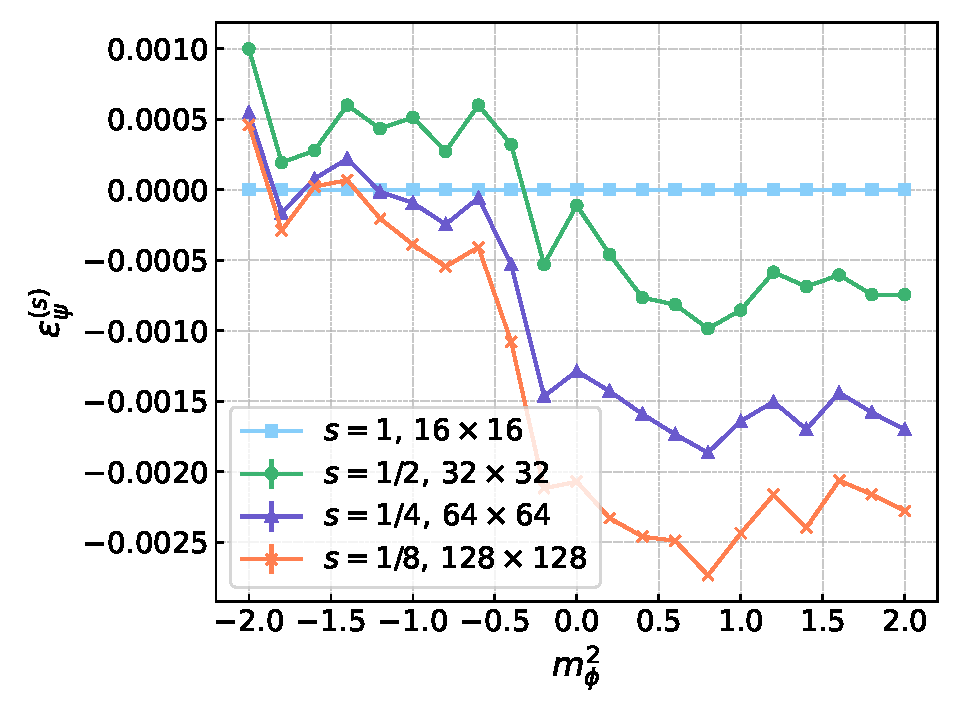
\includegraphics[width=1.0\textwidth]{figures/cooling/mass_scan/deviation_cond.pdf}
        \caption{Chiral condensate}
    \end{subfigure}
    \caption[Relative error in the cooling procedure at tree level.]{Relative error of the absolute magnetisation and chiral condensate in the cooling procedure for various values of the noise fraction $s$.}
    \label{fig:cooling_deviation}
\end{figure}
\begin{figure}[htp]
    \centering
    \begin{subfigure}[b]{0.45\textwidth}
        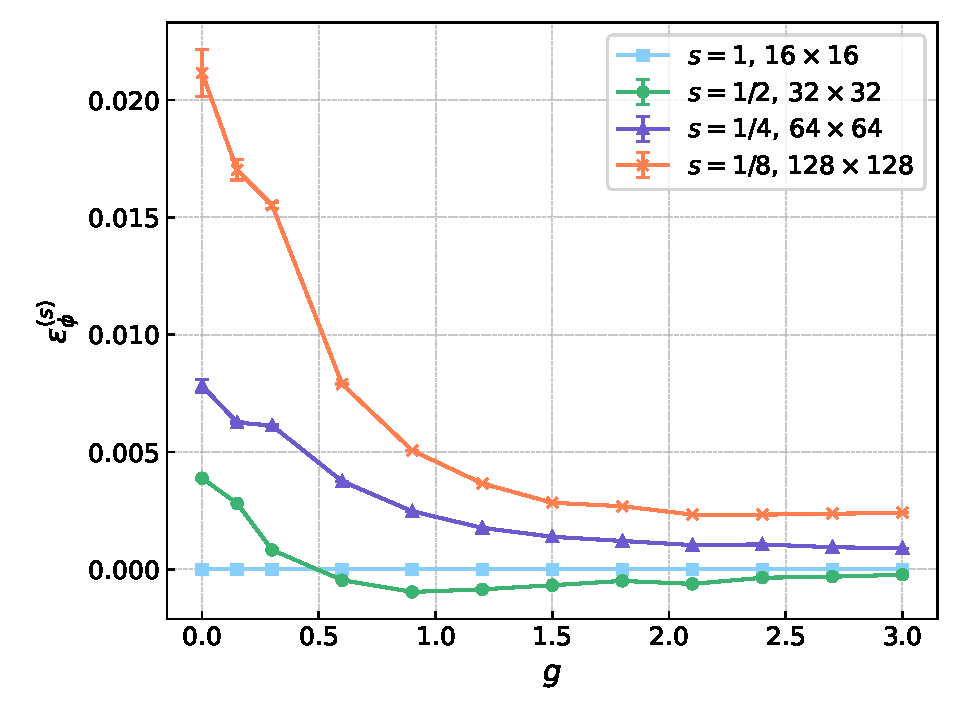
\includegraphics[width=\textwidth]{figures/cooling/yukawa_scan/deviation.pdf}
        \caption{Absolute magnetisation}
    \end{subfigure}
    \begin{subfigure}[b]{0.45\textwidth}
        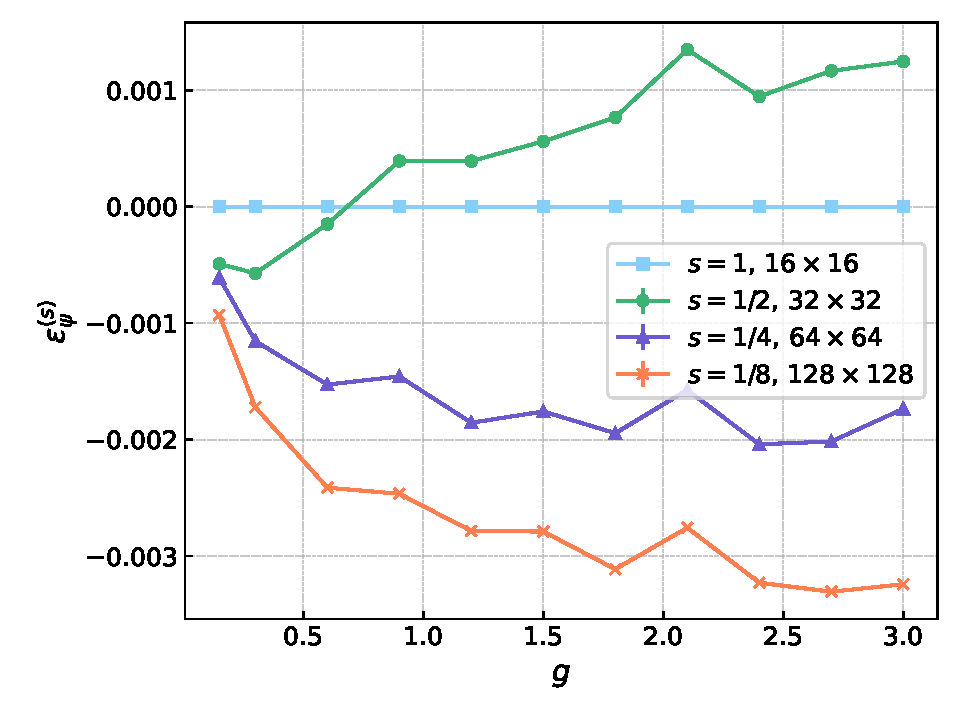
\includegraphics[width=\textwidth]{figures/cooling/yukawa_scan/deviation_cond.pdf}
        \caption{Chiral condensate}
    \end{subfigure}
    \caption[Relative error in the cooling procedure at tree level.]{Relative error of the absolute magnetisation and chiral condensate in the cooling procedure for various values of the noise fraction $s$.}
    \label{fig:cooling_deviation_yukawa}
\end{figure} \\
\newpage
Finally, we also want to look at more complex observables such as the fermionic physical mass and the bosonic renormalised mass. They are reported in figure \ref{fig:cooling_masses}. As one can see, there is a clear deviation for $m_{\phi, r}$ at the third block-spin iteration. This is a systematic deviation because \textcolor{red}{i would say tree level, but I don't think it's the case.}
\begin{figure}[h!]
    \begin{minipage}{0.45\textwidth}
        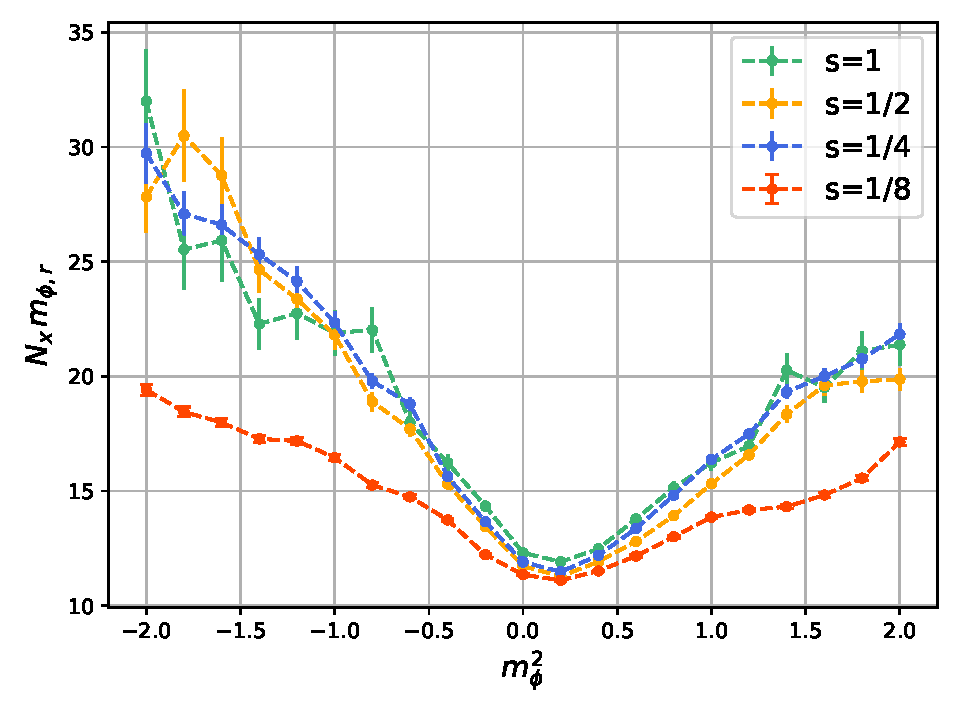
\includegraphics[scale=0.45]{figures/cooling/mass_scan/mphir.pdf}
    \end{minipage}
    \hfill 
    \begin{minipage}{0.45\textwidth}
        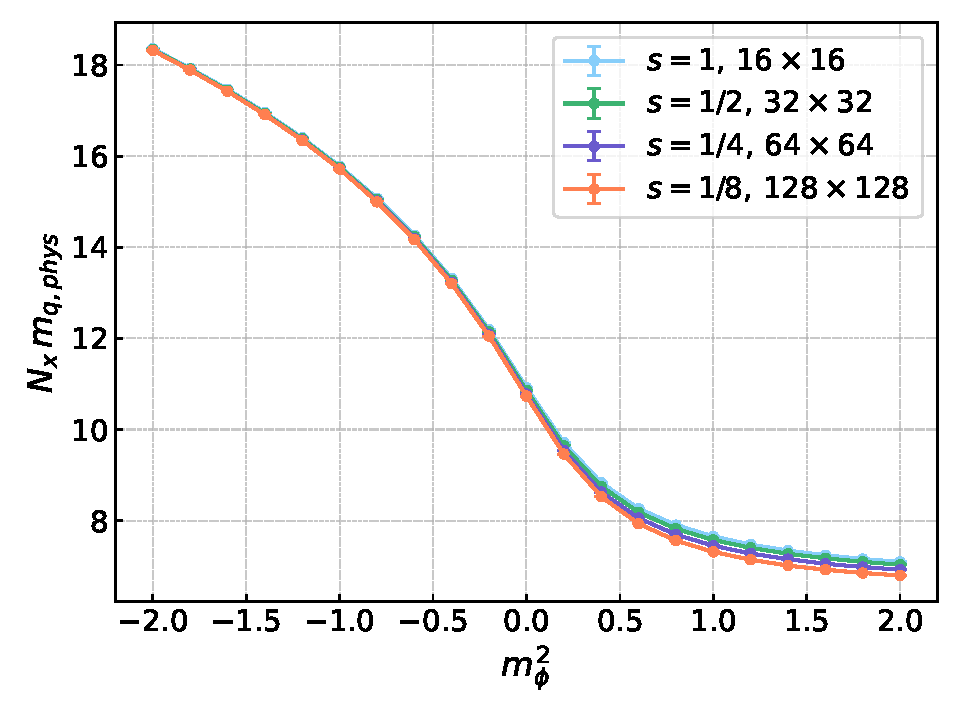
\includegraphics[scale=0.45]{figures/cooling/mass_scan/mqphys.pdf}
    \end{minipage}
    \caption[Masses in the cooling procedure]{Renormalised bosonic mass $m_{\phi, r}$ and pole fermionic mass $m_{q,\text{phys}}$ for various values of the noise fraction $s$.}
    \label{fig:cooling_masses}
\end{figure} 

\newpage

\section{Control over temperature}
\begin{table}
    \centering 
    \begin{tabular}{cccccccccccc}
        \toprule
        $N_t$ & $N_x$ & & s & $a_\text{eff}$ & $T/T_0$ & & $m_\phi^2$ & $\lambda$ & $g$ & $m_q$& $K_\psi$\\
        \midrule
        8 & 8 & & 1 & a & 1 & & 0.6 & 2.0 & g & 1.0 & $K_\psi$\\
        \midrule 
        4 & 8 & & 1 & a & 2 & & 0.6 & 2.0 & 0.3 & 1.0 & $K_\psi$\\
        2 & 8 & & 1 & a & 4 & & 0.6 & 2.0 & 0.3 & 1.0 & $K_\psi$\\
        \midrule
        8 & 16 & & 1/2 & 2a & 2 & & 0.15 & 0.05 & 0.3 & 1.0 & $K_\psi/2$\\
        8 & 32 & & 1/2 & 4a & 4 & & 0.0375 & 0.0125 & 0.3 & 1.0 & $K_\psi/4$\\
        \bottomrule
    \end{tabular}
    \caption{}
    \label{tab:temperature_control_yukawa}
\end{table}
\label{sec:temperature_control}
\begin{figure}
    \centering
    \begin{subfigure}{0.48\textwidth}
        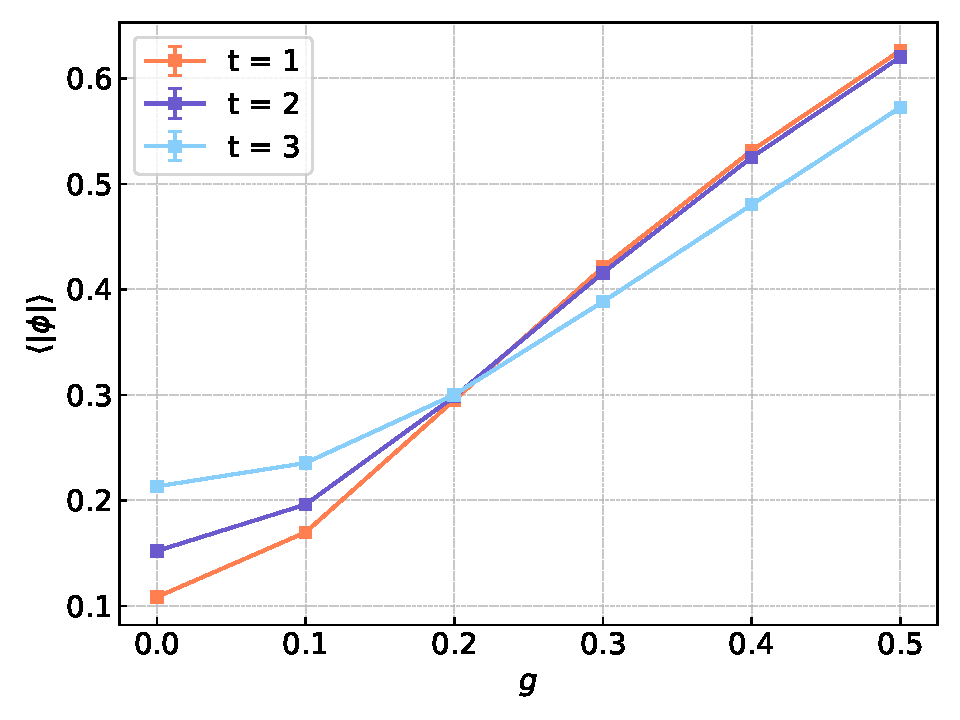
\includegraphics[width=\textwidth]{figures/temperature/temp_mag.pdf}
    \end{subfigure}
    \begin{subfigure}{0.48\textwidth}
        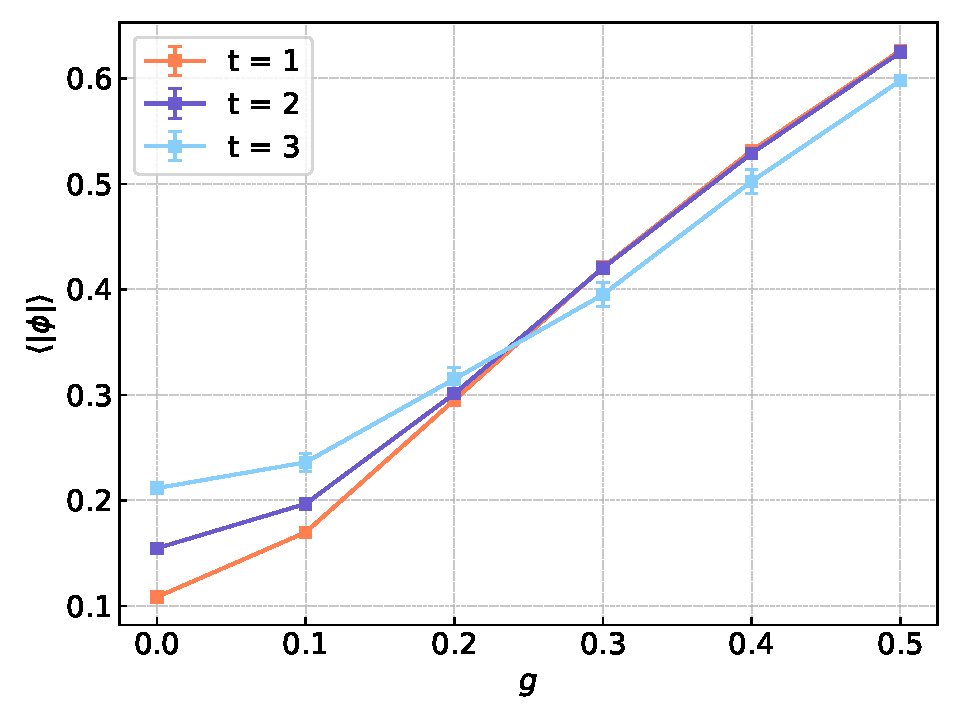
\includegraphics[width=\textwidth]{figures/temperature/temp_mag_coloured.pdf}
    \end{subfigure}
\end{figure}
\begin{figure}
    \centering
    \begin{subfigure}{0.48\textwidth}
        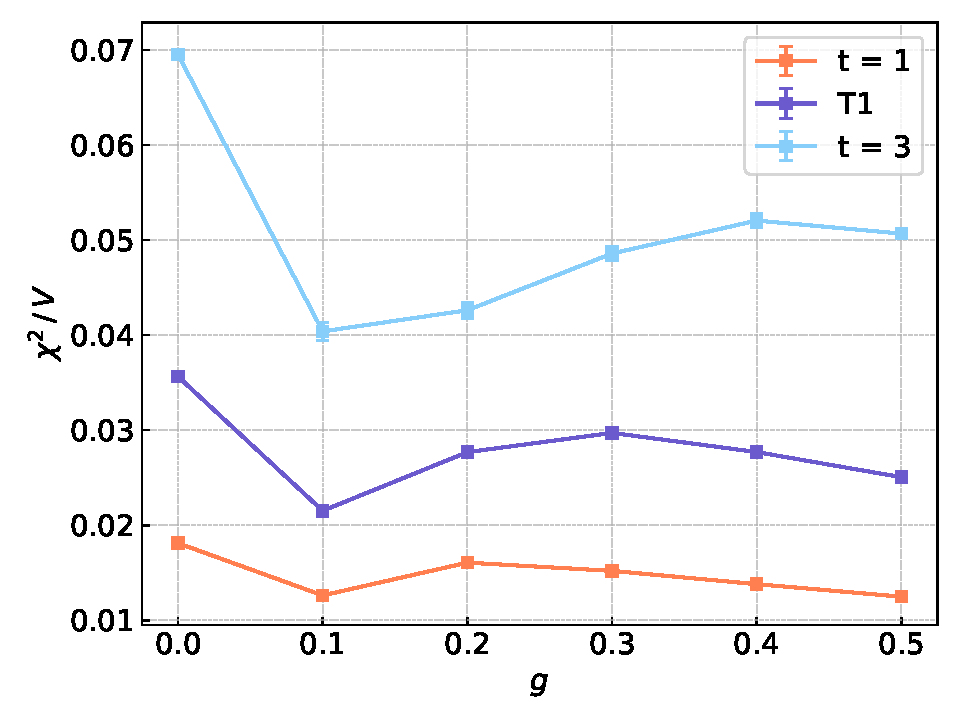
\includegraphics[width=\textwidth]{figures/temperature/temp_chi2.pdf}
    \end{subfigure}
    \begin{subfigure}{0.48\textwidth}
        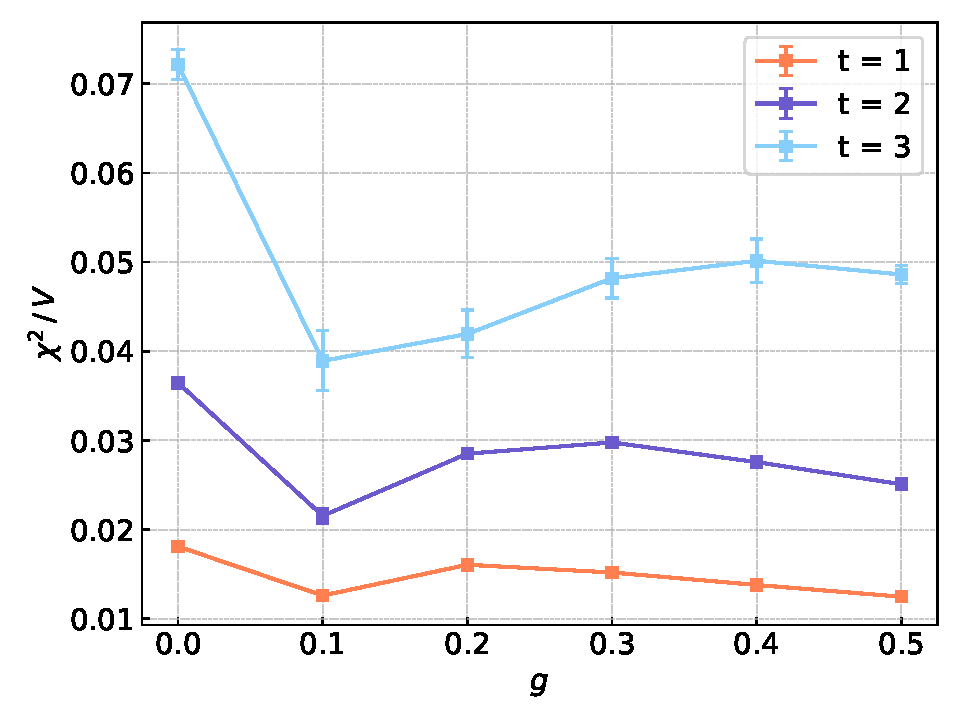
\includegraphics[width=\textwidth]{figures/temperature/temp_chi2_coloured.pdf}
    \end{subfigure}
\end{figure}
